% ============================================================
%  第三卷 第十七章 弹性碰撞（前半：§123–§131 + 习题）
%  底本：高教社中文版第6版；OCR 错误已修正，脚注文本待从纸版补录
%  主要 OCR 修正（行号为 full_merged.md 全局行号）：
%   1. 斜体 ι/下标 t 误读 → l（A_l、δ_l、f_l、S_l，全章统一）；
%      行17324 i^l、(−i)^l 按原书 p461；行17338 (Ω−1)^{l+1} → (−1)^{l+1}；
%   2. 行17271 偏转角句公式错位 → "偏转角 ϑ₁ 和 ϑ₂"（按原书 p459）；
%   3. 行17295 \mathbb{0} → 脚注圈码①；行18077 \textcircled{1} → ①；
%   4. 行17350 e^{ikε} → e^{ikz}；行17370 积分内冗余 "dt" 删除；
%   5. 行17415 散射振幅 𝓘(φ) → f(φ)；行17444 "，⃗*dφ" → "式中"；
%   6. 行17457/17459/17485/17995/18077/18101/18145 等处句中游离的 δ_l 归位；
%   7. 行17485 "接1/rⁿ趋于零" → "按"；行17495 ∑_{l>21} → ∑_{l≫1}；
%   8. 行17544 驻点法积分式原书 p466 印作 e^{±ikr}/r，漏因子 1/k，
%      按"约去公共因子 2πi/k"与(125.3)校核补正为 e^{±ikr}/kr；
%   9. 行17565 "ŝ." → "Ŝ算符"；(125.6)(125.7) 厄米共轭按原书 ^{+}；
%  10. 行17669–17689 §125 末段游离记号归位、"Ifl" → |f|、"复原"；
%  11. 行17707 ψ^(0) 误作粗体 → 正体；行17846 σ_{1r} → σ_{tr}；
%  12. 行17864 §126 习题1 总截面 dσ → σ（原书 p472 即误植，按"得散射总截面"改）；
%  13. 行17870/17874 "H H" → "时"；行17893–17907 习题3 场强分子 a → α（按原书 p473）；
%  14. 行17927 习题4 补回 OCR 漏句 "时上式左边可用渐近式(33.12)和"（p473）；
%  15. 行17946 习题5 被积式/下限乱码 → (r²+a²)^{n/2}、l/k；
%  16. 行17968 习题6 汉克尔渐近式尾部乱码 → (u→∞)；
%  17. 行18004 ∑_i → ∑_l；行18018 "\right]frac" → "]"；
%  18. 行18077 Δθ<<δ → Δθ≪θ；行18083 hl → ħl；行18085 "j^μ̇格" → "严格"；
%  19. 行18104 r^* → rⁿ、下限 νk → l/k；行18135 特征尺度 α → a；
%  20. 行18176 习题3 f=l₀/(iR)：原书 6 版印作 iR（p479），R 未定义，
%      按量纲与结果式 dσ=πl₀²/(βk²)do 校核改 ik；
%  21. 行18220 "\sharp" → "时"；行18254 (128.7) 乱码 → 常数·[e^{i(kr+δ₀)}−e^{−i(kr+δ₀)}]（p481）；
%  22. 行18288 (E+E₀e^{vi}) → (E+|E₀|)（按原书 p482）；
%  23. 行18247 "$c$ 常系数" → "常系数"（按原书 p481）；
%  24. 行18322 (128.13) 乱码 → 按原书 p483 文字型公式照排；
%  25. 行18330 (128.14) 乱码 → U=常数×rⁿe^{−r/a}（按原书 p483）；
%  26. 行18344 (128.15) 乱码重建（常数×{exp[i(kr−lπ/2+δ_l)]−…}），第二指数补 r；
%  27. 行18356 (128.17) (θ−1)^{l+1} → (−1)^{l+1}、h² → ħ²；
%  28. 行18371/18771 行尾扫描噪声 "22"、行18687 "TC" 删除；
%  29. 行18376 ψ 下标乱码 → ψ_散射；行18389 (139.3) → (129.3)；行18391 "与ψek" → 与 e^{ikr}；
%  30. 行18493 (130.4) 被积项乱码 → U(q−q′)a(q′)；行18563 "满定" → "满足"；
%  31. 行18612 ħν → ħv；行18664 下限 νk → l/k；
%  32. 行18793 §131 习题2 玻恩极限 σ=1/2πa²ν² → σ=½π²a²ν²
%      （原书漏 π 的平方，按§126题2 ka≫1 极限值校核）；
%  33. 行18802 {…} → |…|、e^c → e^C（按原书 p494）；行18824 (2) 式左 φ → ψ（原书误植）；
%  34. 行18827 "干π" → ±π；行18832 e^{ikε} → e^{ikz}、F(x) 中 φ → Φ；
%      行18838 第二项乱码 → "复共轭式"（按原书 p495）；行18841 引入 λe^{−λz} → e^{−λx}；
%      行18850–18856 eφ → eΦ；
%  35. §128 行18311–18315 两段重复文字系原书 p482 排印即连排两遍，照排未删。
%  脚注转录（脚注代理）：
%   - 32 处圈码脚注已全部转录为 ootnote{}（按 pages300 页面实况）；
%     页码分布：p472×1、p473×1、p474×1、p477×1、p478×2、p482×1、p483×1、p486×1、
%     p490×1、p492×3、p493×1、p494×1、p496×1、p497×1、p498×3、p500×2、p502×1、
%     p503×2、p504×2、p505×3、p507×2（对照表缺页码者已按页面核实）。
%   - 公式类脚注：p474 Γельфанд-Левитан 渐近式（行内式）；p493 脚注①含编号式
%     (128.5a)（equation*+tag）；p498 脚注②含常数×(1/r)(1/B)[…] 式；
%     p503 脚注②含编号式 (131.7a)（即上文所记"p490 脚注②"，实为 p503，
%     已按原书排入脚注，正文题3仅保留引用）；p504 脚注②含程函积分式。
%   - p507 脚注①中"式(3)"指 §131 题3 解中式 (3)（公式编号沿用原书）。
%  遗留问题：
%   - 图45 属 §108（ch14 已排），本章区间不含；本章插图仅图46/47/48；
%   - 行18077 "Δθ<<δ" 原书扫描不清，按上下文（散射角的不确定度）排作 Δθ≪θ。
% ============================================================
\chapter{弹性碰撞}

\section{散射的一般理论}

经典力学中，两个粒子的碰撞完全取决于它们的速度和碰撞参量（当无相互作用时入射粒子的偏射距离）.量子力学中，这个问题的提法必须改变，因为在定速运动下，轨道概念从而还有碰撞参量已失去意义.在这里，理论的目的只是计算粒子碰撞后偏转（或称被散射到）任一给定角度的概率.本章所讲的弹性碰撞，是指碰撞中的两个粒子保持不变，或者这两个相碰粒子（如果它们是复合粒子的话）的内态保持不变.

弹性碰撞问题和所有的二体问题一样，可以归结为具有折合质量的一个单粒子在力心为固定的场 $U(r)$ 中的散射问题\footnote{在这里我们略去了粒子的自旋-轨道作用（如果粒子具有自旋的话）.有心力场的假定，也排除了例如电子被分子散射等这类过程的考虑.}.这种简化是变换到质心系实现的，在质心系中两粒子的质心保持静止.我们用 $\theta$ 代表这个坐标系中的散射角，它与实验室坐标系中两个粒子的偏转角 $\vartheta_1$ 和 $\vartheta_2$ 之间具有简单的关系，这个实验室系中有一个（第二个）粒子在碰撞以前是静止的：
\begin{equation}
  \tan\vartheta_1=\frac{m_2\sin\theta}{m_1+m_2\cos\theta},\qquad
  \vartheta_2=\frac{1}{2}(\pi-\theta),
\end{equation}
式中 $m_1,m_2$ 是两个粒子的质量（见《力学》，§17）.特别是，当这两个粒子的质量相同时（$m_1=m_2$），简单地有
\begin{equation}
  \vartheta_1=\frac{1}{2}\theta,\qquad
  \vartheta_2=\frac{1}{2}(\pi-\theta)\,;
\end{equation}
和 $\vartheta_1+\vartheta_2=\dfrac{1}{2}\pi$，亦即两粒子以直角散开.

本章中我们总是采用质心为静止的坐标系（除非作特殊的声明），并用 $m$ 代表相碰粒子的折合质量.

沿正 $z$ 轴方向运动的一个自由粒子由平面波所描写，我们把它写成 $\psi=\mathrm{e}^{\mathrm{i}kz}$ 的形式，也就是把它的波函数这样归一化，使其流密度等于粒子速度 $v$.远离散射中心的散射粒子，是由一个 $f(\theta)\mathrm{e}^{\mathrm{i}kr}/r$ 形式的出射球面波所描写，其中的 $f(\theta)$ 是散射角 $\theta$ 的某个函数（$\theta$ 是 $z$ 轴和散射粒子运动方向之间的夹角）.这个函数称为散射振幅.因此，势能为 $U(r)$ 的薛定谔方程之解的精确波函数，在远距离处必须呈下列渐近形式：
\begin{equation}
  \psi\approx\mathrm{e}^{\mathrm{i}kz}+f(\theta)\frac{\mathrm{e}^{\mathrm{i}kr}}{r}.
\end{equation}
散射粒子在单位时间内通过 $\mathrm{d}S=r^2\mathrm{d}o$ 面积元（$\mathrm{d}o$ 是立体角元）的概率等于 $vr^{-2}|f|^2\mathrm{d}S=v|f|^2\mathrm{d}o$\footnote{我们已经假定了入射粒子束是由一个宽（避免衍射效应）而有界的光阑所定义的，这也是散射实验中的实际情况.因此在(123.3)式两项之间不存在干涉；模量平方 $|\psi|^2$ 的取值点处不存在入射波.}.它与入射波的流密度之比为
\begin{equation}
  \mathrm{d}\sigma=|f(\theta)|^2\mathrm{d}o,
\end{equation}
这个量具有面积的量纲，称为散射到 $\mathrm{d}o$ 立体角内的有效截面，或简称为截面.如果令 $\mathrm{d}o=2\pi\sin\theta\,\mathrm{d}\theta$，我们得
\begin{equation}
  \mathrm{d}\sigma=2\pi\sin\theta\,|f(\theta)|^2\mathrm{d}\theta.
\end{equation}
这是散射到 $\theta$ 和 $\theta+\mathrm{d}\theta$ 角度范围内的截面.

对于有心力场 $U(r)$ 中的散射讲来，薛定谔方程之解对 $z$ 轴（入射粒子方向）显然应当是轴对称的.每一个这样的解可以表成运动于该场中的粒子能量给定为 $\hbar^2k^2/2m$ 的许多连续谱波函数的叠加，这些波函数具有不同的轨道角动量值 $l$ 但其 $z$ 分量均为零；这些函数与绕 $z$ 轴的方位角 $\varphi$ 无关，亦即全是轴对称的.因此所需的波函数具有下列形式：
\begin{equation}
  \psi=\sum_{l=0}^{\infty}A_l\mathrm{P}_l(\cos\theta)R_{kl}(r),
\end{equation}
式中 $A_l$ 是常数，$R_{kl}$ 是满足下列方程的径向函数：
\begin{equation}
  \frac{1}{r^2}\frac{\mathrm{d}}{\mathrm{d}r}
  \left(r^2\frac{\mathrm{d}R_{kl}}{\mathrm{d}r}\right)
  +\left[k^2-\frac{l(l+1)}{r^2}-\frac{2m}{\hbar^2}U(r)\right]R_{kl}=0.
\end{equation}
系数 $A_l$ 必须这样来选取，使得(123.6)式的函数在远距离处呈(123.3)的渐近形式.我们将证明这会导致
\begin{equation}
  A_l=\frac{1}{2k}(2l+1)\mathrm{i}^l\exp(\mathrm{i}\delta_l)
\end{equation}
式中的 $\delta_l$ 是函数 $R_{kl}$ 的相移.这个证明还能解决用这些相移表出散射振幅的问题.

$R_{kl}$ 函数的渐近式已由(33.20)式给出：
\begin{equation*}
\begin{aligned}
  R_{kl}&\approx\frac{2}{r}\sin\left(kr-\frac{1}{2}l\pi+\delta_l\right)=\\
  &=\frac{1}{\mathrm{i}r}\left\{(-\mathrm{i})^l
  \exp\left[\mathrm{i}(kr+\delta_l)\right]
  -\mathrm{i}^l\exp\left[-\mathrm{i}(kr+\delta_l)\right]\right\}.
\end{aligned}
\end{equation*}
将上式及(123.8)代入(123.6)，得到波函数的下列渐近式
\begin{equation}
  \psi\approx\frac{1}{2\mathrm{i}kr}\sum_{l=0}^{\infty}(2l+1)
  \mathrm{P}_l(\cos\theta)\left[(-1)^{l+1}\mathrm{e}^{-\mathrm{i}kr}
  +S_l\mathrm{e}^{\mathrm{i}kr}\right],
\end{equation}
其中引入一个记号
\begin{equation}
  S_l=\exp(2\mathrm{i}\delta_l).
\end{equation}
把平面波(34.2)展开，作同样的变换，可得
\begin{equation*}
  \mathrm{e}^{\mathrm{i}kz}\approx\frac{1}{2\mathrm{i}kr}\sum_{l=0}^{\infty}(2l+1)
  \mathrm{P}_l(\cos\theta)\left[(-1)^{l+1}\mathrm{e}^{-\mathrm{i}kr}
  +\mathrm{e}^{\mathrm{i}kr}\right].
\end{equation*}
我们看到，差式 $\psi-\mathrm{e}^{\mathrm{i}kz}$ 中含有 $\mathrm{e}^{-\mathrm{i}kr}$ 因子的各项果真都被消去.这个差式中 $\mathrm{e}^{\mathrm{i}kr}/r$ 前的系数就是散射振幅，我们得
\begin{equation}
  f(\theta)=\frac{1}{2\mathrm{i}k}\sum_{l=0}^{\infty}(2l+1)
  \left[S_l-1\right]\mathrm{P}_l(\cos\theta).
\end{equation}
这个公式解决了用 $\delta_l$ 表达散射振幅的问题（H.~Faxen，J.~Holtsmark，1927）.\footnote{根据相位 $\delta_l$（假定为已知）复原散射势的形状问题十分重要.这个问题是由 И.~М.~Гельфанд，Б.~М.~Левитан 和 В.~А.~Марченко.解决的.他们发现，为了确定 $U(r)$，原则上只需知道 $\delta_0(k)$ 在波数 $k=0$ 到 $k=\infty$ 的整个区域内的函数形状就可以了，如果还有离散（负的）能级 $E_n$ 的话，尚需知道离散态波函数渐近式（当 $r\to\infty$ 时）$R_{n0}\approx a_n\mathrm{e}^{-\kappa_n r}/r$（$\kappa_n=\sqrt{2m|E_n|}/\hbar$）中的系数 $a_n$.根据这些数据确定 $U(r)$，需要求解一个线性积分方程.这个命题的完整讨论见 V.~de~Alfaro，T.~Regge，Potential Scattering，North-Holland，Amsterdam，1965.}

如果 $\mathrm{d}\sigma$ 对所有的角度积分，即得总散射截面 $\sigma$，它等于粒子被散射的总概率（单位时间内）与入射波概率流密度之比.把(123.11)代入下列积分式：
\begin{equation*}
  \sigma=2\pi\int_0^{\pi}|f(\theta)|^2\sin\theta\,\mathrm{d}\theta.
\end{equation*}
考虑到 $l$ 值不同的勒让德多项式是正交的，而
\begin{equation*}
  \int_0^{\pi}P_l^2(\cos\theta)\sin\theta\,\mathrm{d}\theta
  =\frac{2}{2l+1},
\end{equation*}
得到总截面
\begin{equation}
  \sigma=\frac{4\pi}{k^2}\sum_{l=0}^{\infty}(2l+1)\sin^2\delta_l.
\end{equation}
这个求和式中的每一项就是对轨道角动量给定为 $l$ 的散射粒子而言的分波截面 $\sigma_l$.注意 $\sigma_l$ 的最大可能值为
\begin{equation}
  \sigma_{l,\mathrm{max}}=\frac{4\pi}{k^2}(2l+1)
\end{equation}
上式与(34.5)式比较后可知，角动量为 $l$ 的散射粒子数可以比入射束中的这种粒子数大四倍.这是一种纯粹的量子效应，它来自散射粒子和未被散射粒子间的干涉.

今后还要用到分波散射振幅 $f_l$，它定义为以下展开式中的系数：
\begin{equation}
  f(\theta)=\sum_l(2l+1)f_l\mathrm{P}_l(\cos\theta).
\end{equation}
按(123.11)，它和相位 $\delta_l$ 的关系为
\begin{equation}
  f_l=\frac{1}{2\mathrm{i}k}(S_l-1)
  =\frac{1}{2\mathrm{i}k}\left(\mathrm{e}^{2\mathrm{i}\delta_l}-1\right),
\end{equation}
而分波截面为
\begin{equation}
  \sigma_l=4\pi(2l+1)|f_l|^2.
\end{equation}

\setcounter{equation}{0}\renewcommand{\theequation}{\arabic{section}.\arabic{equation}}%

\section{一般公式的研究}

以上所得的公式，原则上适用于任一场 $U(r)$ 中的散射，该场在无穷远处等于零.这些公式的应用，只归结为对式中出现的相位 $\delta_l$ 的性质的考察.

为了估计出 $l$ 值很大时的相位 $\delta_l$ 的数量级，我们可以利用 $l$ 很大时运动为准经典的事实（见§49）.波函数的相位此时由以下积分确定：
\begin{equation*}
  \int_{r_0}^{r}\sqrt{k^2-\frac{(l+1/2)^2}{r^2}
  -\frac{2mU(r)}{\hbar^2}}\,\mathrm{d}r+\frac{1}{4}\pi,
\end{equation*}
其中 $r_0$ 是根号内表式的一个根（$r>r_0$ 是运动的经典允许区）.从上式中减去以下自由运动波函数的相位：
\begin{equation*}
  \int_{r_0}^{r}\sqrt{k^2-\frac{(l+1/2)^2}{r^2}}\,\mathrm{d}r
  +\frac{1}{4}\pi,
\end{equation*}
并令 $r\to\infty$，按定义即得 $\delta_l$.对于很大的 $l$，$r_0$ 也变得很大，因此 $U(r)$ 在整个积分区内都很小，我们近似地得
\begin{equation}
  \delta_l=-\int_{r_0}^{\infty}
  \frac{mU(r)\,\mathrm{d}r}{\hbar^2\sqrt{k^2-\frac{(l+1/2)^2}{r^2}}}.
\end{equation}
此积分（如果收敛）的数量级为
\begin{equation}
  \delta_l\sim\frac{mU(r_0)r_0}{k\hbar^2},
\end{equation}
$r_0$ 的数量级为 $r_0\sim l/k$.

如果 $U(r)$ 在无穷远处按 $1/r^n$ 趋于零（$n>1$），则积分(124.1)收敛而相位 $\delta_l$ 为有限.反之，如果 $n\leqslant1$，积分发散，从而相位 $\delta_l$ 为无穷大.这一点对任意的 $l$ 都能成立，因为积分(124.1)的收敛或发散依赖于 $U(r)$ 在 $r$ 很大处的行为，然而在远距离处（该处的 $U(r)$ 场已很弱），径向运动对所有的 $l$ 讲来都是准经典的.我们将在下面看到，(123.11)和(123.12)式当 $\delta_l$ 无穷大时将作怎样的解释.

我们先考虑总截面级数表式(123.12)的收敛性.如果考虑到 $U(r)$ 比 $1/r$ 递降得更快，由(124.1)式可知，$l$ 大时相位 $\delta_l\ll1$.因此可令 $\sin^2\delta_l\approx\delta_l^2$，(123.12)式高次项之和就具有 $\sum_{l\gg1}l\delta_l^2$ 的数量级.根据级数收敛性的积分准则，我们知道，只要积分式 $\int^{\infty}l\delta_l^2\,\mathrm{d}l$ 收敛，则所考虑的级数就是收敛的.把(124.2)式代入并把 $l$ 换成 $kr_0$ 后，即得下列积分式：
\begin{equation*}
  \int^{\infty}U^2(r_0)r_0^3\,\mathrm{d}r_0,
\end{equation*}
如果 $U(r)$ 在无穷远处按 $1/r^n$ 衰减而 $n>2$，这个积分收敛，从而总截面为有限.反之，如果场 $U(r)$ 衰减得不比 $1/r^2$ 快，总截面就变成无穷大.这一点的物理原因是，当场只是随距离缓慢地衰减时，小角度散射的概率变得很大.我们可以回顾一下经典力学中的有关情形，当粒子以很大的但是有限的碰撞参量 $\rho$ 通过任一势场（这个场只当 $r\to\infty$ 时才等于零）时，总是要偏转一个很小的但是并不等于零的角度，因此不管 $U(r)$ 的衰减规律如何，它的总散射截面总是等于无穷大\footnote{这反映在经典力学中确定总截面的积分 $\int 2\pi\rho\,\mathrm{d}\rho$ 是发散的.}.这种论证在量子力学中并不成立，因为当我们讲到散射到某个角度时，这个角度必须比粒子运动方向的不确定度大得多.如果碰撞参量的已知精确度为 $\Delta\rho$，那么它所引起的动量横向分量的不确定度为 $\hbar/\Delta\rho$，亦即角度的不确定度为 $\sim\hbar/(mv\Delta\rho)$.

鉴于 $U(r)$ 衰减缓慢时小角度散射占有重要的地位，这就自然地产生了这样的一个问题，$U(r)$ 即使比 $1/r^2$ 衰减得更快，$\theta=0$ 的散射振幅有没有可能仍是发散的？我们令(123.11)中的 $\theta=0$，对后面的项讲来它们的和与 $\sum_{l\gg1}l\delta_l$ 成正比.正如上段中所做的论证那样，当判别这个和是否收敛时，最后我们得到以下积分：
\begin{equation*}
  \int^{\infty}U(r_0)r_0^2\,\mathrm{d}r_0,
\end{equation*}
当 $U(r)\sim1/r^n$ 而 $n\leqslant3$ 时，此积分发散.由此可见，势场的衰减不快于 $1/r^3$ 时，$\theta=0$ 处的散射振幅变成无穷大.

最后，我们来考虑相位 $\delta_l$ 本身等于无穷大的情形，它发生于 $U(r)\sim1/r^n$ 而 $n\leqslant1$.根据以上所得的结论显然可以知道，当场衰减得这样慢的时候，总截面以及 $\theta=0$ 的散射振幅都将等于无穷大.但还留下一个如何计算 $\theta\neq0$ 的 $f(\theta)$ 问题.

首先应该注意的是，我们有下列公式\footnote{这个公式就是 $\delta$ 函数的勒让德多项式展开，上式两边乘以 $\sin\theta\,\mathrm{P}_l(\cos\theta)$ 并对 $\mathrm{d}\theta$ 积分后即可得到直接验证.其中偶函数 $\delta(x)$ 的积分式 $\int_0^{\infty}\delta(x)\,\mathrm{d}x$ 取为 1/2.}
\begin{equation}
  \sum_{l=0}^{\infty}(2l+1)\mathrm{P}_l(\cos\theta)
  =4\delta(1-\cos\theta).
\end{equation}
换句话说，只要 $\theta\neq0$ 这个和就等于零.所以对(123.11)式的散射振幅讲来，$\theta\neq0$ 时我们可以略去每项方括号内的1，留下
\begin{equation}
  f(\theta)=\frac{1}{2\mathrm{i}k}\sum_{l=0}^{\infty}(2l+1)
  \mathrm{P}_l(\cos\theta)\mathrm{e}^{2\mathrm{i}\delta_l}.
\end{equation}
如果上式右边乘一常数因子 $\mathrm{e}^{-2\mathrm{i}\delta_0}$ 截面不会发生改变，因为它是由模量平方 $|f(\theta)|^2$ 确定的，此时复函数 $f(\theta)$ 的相位只是改变了一个不重要的常数.另一方面，把差 $\delta_l-\delta_0$ 表成(124.1)式那样，$U(r)$ 的积分发散性就被消去，只留下一个有限的量.因此在所考虑的情形下，我们可以采用下列公式计算散射振幅
\begin{equation}
  f(\theta)=\frac{1}{2\mathrm{i}k}\sum_{l=0}^{\infty}(2l+1)
  \mathrm{P}_l(\cos\theta)\mathrm{e}^{2\mathrm{i}(\delta_l-\delta_0)}.
\end{equation}

\begin{xiti}
\setcounter{equation}{0}\renewcommand{\theequation}{\arabic{equation}}%

\noindent{\heiti 习题}\quad 在二维情况下，试用相移表出散射振幅.场为 $U=U(\rho)$，$\rho=\sqrt{x^2+z^2}$，入射粒子流沿 $z$ 轴方向.

解：在二维情况下，在散射点远处的波函数是平面波和柱面波的叠加
\begin{equation}
  \psi=\mathrm{e}^{\mathrm{i}kz}
  +f(\varphi)\frac{\mathrm{e}^{\mathrm{i}k\rho}}{\sqrt{-\mathrm{i}\rho}}.
\end{equation}
式中 $\varphi$ 是散射方向与 $z$ 轴的夹角，$f(\varphi)$ 是散射振幅，它在二维情况下的量纲是长度的平方根.在根号下面引进的因子 $-\mathrm{i}=\exp(-\mathrm{i}\pi/2)$ 是为了简化以后的分式.沿 $y$ 轴单位长度的散射截面为
\begin{equation*}
  \mathrm{d}\sigma=|f|^2\mathrm{d}\varphi.
\end{equation*}
它的量纲是长度.

应当把波函数展开为在 $y$ 轴方向上具有确定的角动量分量、形如 $Q_m(\rho)\mathrm{e}^{\mathrm{i}m\varphi}$ 的函数，这些函数在远离散射点处的形式与在§34所得的自由运动的展开式只相差一些相移
\begin{equation*}
  Q_m(\rho)\approx\mathrm{i}^m\sqrt{\frac{2}{\pi k\rho}}
  \sin\left[k\rho-\frac{\pi}{2}\left(m-\frac{1}{2}\right)+\delta_m\right],
\end{equation*}
式中 $\delta_m=\delta_{-m}$.利用§34中各题中的平面波的展开式按本节的方法展开，我们发现，渐近行为如(1)式的函数可以用级数表出：
\begin{equation*}
  \psi=\sum_{m=-\infty}^{\infty}\mathrm{e}^{\mathrm{i}\delta_m}
  Q_m(\rho)\mathrm{e}^{\mathrm{i}m\varphi},
\end{equation*}
而散射振幅等于
\begin{equation}
  f(\varphi)=\frac{1}{\mathrm{i}\sqrt{2\pi k}}
  \sum_{m=-\infty}^{\infty}\left(\mathrm{e}^{2\mathrm{i}\delta_m}-1\right)
  \mathrm{e}^{\mathrm{i}m\varphi}.
\end{equation}
积分得总截面为
\begin{equation}
  \sigma=\int_0^{2\pi}|f|^2\mathrm{d}\varphi=\sum_m\sigma_m,
  \quad\text{式中}\ \sigma_m=\sigma_{-m}=\frac{4}{k}\sin^2\delta_m.
\end{equation}
不难验证二维情形下的光学定理为
\begin{equation*}
  \operatorname{Im}f(0)=\sqrt{\frac{k}{8\pi}}\,\sigma,
\end{equation*}
参见下节(125.9)式.

\end{xiti}

\section{散射的幺正条件}

任意场（不一定是有心力场）中的散射振幅都能满足来自一般物理要求的某些关系式.

对任意场中的弹性散射讲来，波函数在远距离处的渐近式为
\begin{equation}
  \psi\approx\mathrm{e}^{\mathrm{i}kr\boldsymbol{n}\cdot\boldsymbol{n}'}
  +\frac{1}{r}f(\boldsymbol{n},\boldsymbol{n}')\mathrm{e}^{\mathrm{i}kr}.
\end{equation}
这个公式与(123.3)不同之处在于，现在的散射振幅依赖于两个单位矢量的方向，入射粒子的方向（$\boldsymbol{n}$）以及散射粒子的方向（$\boldsymbol{n}'$），而不光是依赖于这两个方向的夹角.

入射方向 $\boldsymbol{n}$ 不同的各种(125.1)式的函数，它们的任意线性组合仍代表某一可能的散射过程.把(125.1)式乘以任意系数 $F(\boldsymbol{n})$ 并对 $n$ 的各个方向（立体角元 $\mathrm{d}o$）积分后，就能把这样的线性组合写成以下积分形式：
\begin{equation}
  \int F(\boldsymbol{n})
  \mathrm{e}^{\mathrm{i}kr\boldsymbol{n}\cdot\boldsymbol{n}'}\,\mathrm{d}o
  +\frac{\mathrm{e}^{\mathrm{i}kr}}{r}
  \int F(\boldsymbol{n})f(\boldsymbol{n},\boldsymbol{n}')\,\mathrm{d}o.
\end{equation}
由于距离 $r$ 任意大，第一个积分中的因子
$\mathrm{e}^{\mathrm{i}kr\boldsymbol{n}\cdot\boldsymbol{n}'}$
是变矢量 $n$ 的方向的急剧振荡函数.因此该积分主要由指数极值（此时 $\boldsymbol{n}=\pm\boldsymbol{n}'$）附近的 $n$ 值所确定.在 $\boldsymbol{n}=\pm\boldsymbol{n}'$ 的邻域中，因子 $F(\boldsymbol{n})\approx F(\pm\boldsymbol{n}')$ 可以拿出积分号外，然后积分得\footnote{计算这个积分时可把积分路径弯向 $\mu=\cos\theta$ 变量（$\theta$ 是 $\boldsymbol{n}$ 和 $\boldsymbol{n}'$ 间的夹角）的上半复平面，保持它的两端 $\mu=\pm1$ 不动.远离这两个端点时，$\mathrm{e}^{\mathrm{i}kr\mu}$ 函数就很快地衰减.}：
\begin{equation*}
  2\pi\mathrm{i}F(-\boldsymbol{n}')\frac{\mathrm{e}^{-\mathrm{i}kr}}{kr}
  -2\pi\mathrm{i}F(\boldsymbol{n}')\frac{\mathrm{e}^{\mathrm{i}kr}}{kr}
  +\frac{\mathrm{e}^{\mathrm{i}kr}}{r}
  \int f(\boldsymbol{n},\boldsymbol{n}')F(\boldsymbol{n})\,\mathrm{d}o.
\end{equation*}
约去公共因子 $2\pi\mathrm{i}/k$，上式可写成简洁的算符形式
\begin{equation}
  \frac{\mathrm{e}^{-\mathrm{i}kr}}{r}F(-\boldsymbol{n}')
  -\frac{\mathrm{e}^{\mathrm{i}kr}}{r}\hat{S}F(\boldsymbol{n}'),
\end{equation}
式中
\begin{equation}
  \hat{S}=1+2\mathrm{i}k\hat{f},
\end{equation}
$\hat{f}$ 是由下式定义的积分算符：
\begin{equation}
  \hat{f}F(\boldsymbol{n}')=\frac{1}{4\pi}
  \int f(\boldsymbol{n},\boldsymbol{n}')F(\boldsymbol{n})\,\mathrm{d}o.
\end{equation}
$\hat{S}$ 算符称为散射算符（或散射矩阵）或者简称为 $S$ 矩阵，它是由海森伯首先引入的（1943）.

(125.3)中的第一项代表射向力心的波，第二项代表离开力心的波.弹性散射中，粒子数守恒可表为入射波和出射波的流密度相等.换句话说，这两个波的归一化应该相同.为此，散射算符必须是幺正的（§12），也就是说，必须有
\begin{equation}
  \hat{S}\hat{S}^{+}=1,
\end{equation}
或者把(125.4)式代入上式并互乘
\begin{equation}
  \hat{f}-\hat{f}^{+}=2\mathrm{i}k\hat{f}\hat{f}^{+}.
\end{equation}
最后，利用定义(125.5)，我们可以把散射的幺正条件写成以下形式：
\begin{equation}
  f(\boldsymbol{n},\boldsymbol{n}')-f^{*}(\boldsymbol{n}',\boldsymbol{n})
  =\frac{\mathrm{i}k}{2\pi}
  \int f(\boldsymbol{n},\boldsymbol{n}'')f^{*}(\boldsymbol{n}',\boldsymbol{n}'')\,
  \mathrm{d}o''.
\end{equation}
$\boldsymbol{n}=\boldsymbol{n}'$ 时上式右边的积分正是散射总截面
$\sigma=\int|f(\boldsymbol{n},\boldsymbol{n}'')|^2\,\mathrm{d}o''$.
上式左边的差值此时可以化成振幅 $f(\boldsymbol{n},\boldsymbol{n})$ 的虚部.这样，我们就得到了弹性散射总截面和零角度散射振幅虚部之间的普遍关系式：
\begin{equation}
  \operatorname{Im}f(\boldsymbol{n},\boldsymbol{n})=\frac{k}{4\pi}\sigma,
\end{equation}
此式称为散射的光学定理.

散射振幅的另一个普遍性质，可以根据时间反演对称性的要求导出.在量子力学中，这种对称性表述为：如函数 $\psi$ 描述任一可能态，那么它的复共轭函数 $\psi^{*}$ 也对应于某一可能态（§18）.因此(125.3)式的复共轭波函数
\begin{equation*}
  \frac{\mathrm{e}^{\mathrm{i}kr}}{r}F^{*}(-\boldsymbol{n}')
  -\frac{\mathrm{e}^{-\mathrm{i}kr}}{r}\hat{S}^{*}F^{*}(\boldsymbol{n}')
\end{equation*}
也描述某种可能的散射过程.我们通过令
$-\hat{S}^{*}F^{*}(\boldsymbol{n}')=\Phi(-\boldsymbol{n}')$
定义一个新的任意函数.利用算符 $\hat{S}$ 的幺正性就得
\begin{equation*}
  F^{*}(\boldsymbol{n}')
  =-\left(\hat{S}^{*}\right)^{-1}\Phi(-\boldsymbol{n}')
  =-\hat{\tilde{S}}\,\Phi(-\boldsymbol{n}')
\end{equation*}
引入改变矢量 $\boldsymbol{n}$ 和 $\boldsymbol{n}'$ 符号的坐标反演算符 $\hat{P}$，则可写出
\begin{equation*}
  F^{*}(-\boldsymbol{n}')=\hat{P}F^{*}(\boldsymbol{n}')
  =-\hat{P}\hat{\tilde{S}}\,\Phi(\boldsymbol{n}'),
\end{equation*}
从而得到下列时间反演波函数：
\begin{equation*}
  \frac{\mathrm{e}^{-\mathrm{i}kr}}{r}\Phi(-\boldsymbol{n}')
  -\frac{\mathrm{e}^{\mathrm{i}kr}}{r}
  \hat{P}\hat{\tilde{S}}\hat{P}\,\Phi(\boldsymbol{n}').
\end{equation*}
此式必须和原先的波函数(125.3)实质上相同.比较后表明，它导致下列条件
\begin{equation}
  \hat{P}\hat{\tilde{S}}\hat{P}=\hat{S},
\end{equation}
此时两个波函数只是在任意函数的记号上有差别.

把算符等式(125.10)变换成矩阵等式后，即得散射振幅的相应关系式.转置使初末态矢量 $\boldsymbol{n}$ 和 $\boldsymbol{n}'$ 对调，反演则改变它们的符号.因此有
\begin{equation}
  S(\boldsymbol{n},\boldsymbol{n}')
  =S(-\boldsymbol{n}',-\boldsymbol{n}).
\end{equation}
也就是
\begin{equation}
  f(\boldsymbol{n},\boldsymbol{n}')
  =f(-\boldsymbol{n}',-\boldsymbol{n}).
\end{equation}
这个关系式（称为倒易定理）表达了这样一个明显结果：两个互为时间反演的散射过程具有相等的振幅.时间反演把初末态对调并把态中的粒子运动方向变成反方向.

对于有心力场中的散射，以上所得的普遍公式可以简化.这种情形下的振幅 $f(\boldsymbol{n},\boldsymbol{n}')$ 只与 $\boldsymbol{n}$ 和 $\boldsymbol{n}'$ 的夹角 $\theta$ 有关.因此(125.12)变成了一个恒等式.幺正条件(125.8)变成
\begin{equation}
  \operatorname{Im}f(\theta)=\frac{k}{4\pi}
  \int f(\gamma)f^{*}(\gamma')\,\mathrm{d}o'',
\end{equation}
式中 $\gamma,\gamma'$ 是 $\boldsymbol{n},\boldsymbol{n}'$ 与空间中某一固定方向 $\boldsymbol{n}''$ 间的夹角.如果 $f(\theta)$ 采用展开式(123.14)，应用球谐函数的加法定理(c.10)，可从(125.13)式中得出分波振幅的下列关系式：
\begin{equation}
  \operatorname{Im}f_l=k|f_l|^2.
\end{equation}
这个公式也可直接从(123.15)式导出，按该式有 $|2\mathrm{i}kf_l+1|^2=1$.在有心力场中散射的情形下，光学定理(125.9)也很易从(123.11)和(123.12)式直接导出.

把(125.14)式改写成 $\operatorname{Im}(1/f_l)=-k$ 后，即可看出振幅 $f_l$ 必须具有下列形式：
\begin{equation}
  f_l=\frac{1}{g_l-\mathrm{i}k},
\end{equation}
式中的 $g_l=g_l(k)$ 是一个实量；它和相位 $\delta_l$ 的关系为
\begin{equation}
  g_l=k\cot\delta_l.
\end{equation}
以后我们要多次用到这个振幅表达式.

我们来考察一下（对有心力场中的散射）以上定义的散射算符和§123理论中所述各量的关系.

由于轨道角动量在有心力场中是守恒的，散射算符和角动量算符对易.换句话说，$S$ 矩阵在 $l$ 表象中是对角的，又由于 $\hat{S}$ 算符是幺正的，它的本征值模量必等于1，亦即必具有 $\mathrm{e}^{2\mathrm{i}\delta_l}$ 的形式，而 $\delta_l$ 为实数.很易看出，这些 $\delta_l$ 和波函数的相移是一样的，使得 $S$ 矩阵的本征值就是(123.10)中定义的 $S_l$.算符 $\hat{f}=(\hat{S}-1)/2\mathrm{i}k$ 的本征值就是分波振幅(123.15).实际上，如果我们把函数 $F(\boldsymbol{n})$ 取作 $\mathrm{P}_l(\cos\theta)$［从而
$F(-\boldsymbol{n})=\mathrm{P}_l(-\cos\theta)=(-1)^l\mathrm{P}_l(\cos\theta)$］，
波函数(125.3)应该等于(123.9)中一个求和项所代表的薛定谔方程之解.因此有
\begin{equation*}
  \hat{S}\,\mathrm{P}_l(\cos\theta)=S_l\,\mathrm{P}_l(\cos\theta).
\end{equation*}
对于沿 $z$ 轴入射的平面波讲来，(125.3)中的函数 $F(\boldsymbol{n})$ 就是δ函数 $F=4\delta(1-\cos\theta)$，其中的 $\theta$ 是 $\boldsymbol{n}$ 和 $z$ 轴的夹角，这里定义的δ函数可参考§124中对(124.3)所加的注，δ函数前所选的系数是这样的，当它代入定义(125.5)式的右边时正好可以得出 $f(\theta)$，这时 $\theta$ 是 $\boldsymbol{n}'$ 和 $z$ 轴的夹角.把这个δ函数表成(124.3)式的形状：
\begin{equation}
  F=4\delta(1-\cos\theta)=\sum_{l=0}^{\infty}(2l+1)
  \mathrm{P}_l(\cos\theta)
\end{equation}
再把算符 $\hat{f}$ 作用在它上面，于是，正如所预期的，我们即可得到，形如(123.14)式的散射振幅.

最后，还应添加下面的说明.从数学观点看来，幺正条件(125.8)式说明了这样一个事实，并不是所有预先给定的函数 $f(\boldsymbol{n},\boldsymbol{n}')$ 都能成为某个场中的散射振幅.特别是，并不是所有的函数 $f(\theta)$ 都能成为某个有心力场中的散射振幅.根据(125.13)式，它的虚部和实部之间必须满足一定的关系.如果把它写成 $f(\theta)=|f|\mathrm{e}^{\mathrm{i}\alpha}$，当模量 $|f|$ 与所有角度的关系给定以后，(125.13)式就给出一个积分方程，由它原则上可解出未知的相位 $\alpha(\theta)$.换句话说，知道了散射截面（即模量平方 $|f|^2$）与所有角度的关系以后，就可在原则上复原该散射振幅.但是这样的复原缺乏唯一性，它可以相差一个以下的变换式
\begin{equation}
  f(\theta)\to-f^{*}(\theta)
\end{equation}
上式能使(125.13)式保持不变［当然也使截面 $|f|^2$ 保持不变.(125.18)式的变换等价于(123.11)中所有相位 $\delta_l$ 同时变号］.但是，这样的非唯一性是可以消除的，只要把散射振幅看作既是角度的函数也是能量的函数.以后将看到（§128，§129），作为能量函数的振幅，它的解析性质对(125.18)式的变换不是不变的.

\section{玻恩公式}

在一个极为重要的情形下，即当散射场本身可以看作微扰时，能够得到散射截面的一般计算公式\footnote{在§123中导出的普遍性理论中，这个近似相当于所有 $\delta_l$ 全都很小时的情形，并且要求这些相位都可从以势能为微扰的薛定谔方程中算出来（见例题4）.}.§45中已经证明，当以下两条件之一成立时，即有当作微扰的可能：
\begin{equation}
  |U|\ll\frac{\hbar^2}{ma^2}
\end{equation}
以及
\begin{equation}
  |U|\ll\frac{\hbar v}{a}=\frac{\hbar^2}{ma^2}ka,
\end{equation}
式中的 $a$ 是场 $U(r)$ 的作用范围，$U$ 是该场主要区域内的场值的数量级.当第一个条件得到满足时，这个近似对所有的速度都能成立；第二个条件表明，它对足够快的粒子总是适用的.

根据§45，我们把波函数取成 $\psi=\psi^{(0)}+\psi^{(1)}$ 的形式，式中的
$\psi^{(0)}=\mathrm{e}^{\mathrm{i}\boldsymbol{k}\cdot\boldsymbol{r}}$
对应于波矢为 $\boldsymbol{k}=\boldsymbol{p}/\hbar$ 的入射粒子.根据(45.3)式我们有
\begin{equation}
  \psi^{(1)}(x,y,z)=-\frac{m}{2\pi\hbar^2}
  \int U(x',y',z')\mathrm{e}^{\mathrm{i}(\boldsymbol{k}\cdot\boldsymbol{r}'+kR)}
  \frac{\mathrm{d}V'}{R}.
\end{equation}
取散射中心为原点，我们从原点到 $\psi^{(1)}$ 值的计算点引一径矢量 $\boldsymbol{R}_0$，把沿 $\boldsymbol{R}_0$ 的单位矢量记作 $\boldsymbol{n}'$；设体积元 $\mathrm{d}V'$ 的径矢量为 $\boldsymbol{r}'$，则有 $\boldsymbol{R}=\boldsymbol{R}_0-\boldsymbol{r}'$.在远离中心处，$R_0\gg r'$，因而
\begin{equation*}
  R=|\boldsymbol{R}_0-\boldsymbol{r}'|
  \approx R_0-\boldsymbol{r}'\cdot\boldsymbol{n}',
\end{equation*}
把它代入(126.3)，我们得 $\psi^{(1)}$ 的下列渐近式：
\begin{equation*}
  \psi^{(1)}\approx-\frac{m}{2\pi\hbar^2}
  \frac{\mathrm{e}^{\mathrm{i}kR_0}}{R_0}
  \int U(\boldsymbol{r}')
  \mathrm{e}^{\mathrm{i}(\boldsymbol{k}-\boldsymbol{k}')\cdot\boldsymbol{r}'}
  \,\mathrm{d}V'
\end{equation*}
（式中 $\boldsymbol{k}'=k\boldsymbol{n}'$ 是散射后粒子的波矢量）.上式和(123.3)式给出的散射振幅相比较，求得后者的表式为
\begin{equation}
  f=-\frac{m}{2\pi\hbar^2}
  \int U\mathrm{e}^{-\mathrm{i}\boldsymbol{q}\cdot\boldsymbol{r}}\,\mathrm{d}V,
\end{equation}
式中已经变换了积分变量并且引进了矢量
\begin{equation}
  \boldsymbol{q}=\boldsymbol{k}'-\boldsymbol{k},
\end{equation}
$\boldsymbol{q}$ 的绝对值是
\begin{equation}
  q=2k\sin\frac{\theta}{2}
\end{equation}
其中 $\theta$ 是 $\boldsymbol{k}$ 和 $\boldsymbol{k}'$ 的夹角，也就是散射角.

最后，把散射振幅的模量加以平方，即得下列散射到 $\mathrm{d}o$ 立体角元中的截面表式：
\begin{equation}
  \mathrm{d}\sigma=\frac{m^2}{4\pi^2\hbar^4}
  \left|\int U\mathrm{e}^{-\mathrm{i}\boldsymbol{q}\cdot\boldsymbol{r}}\,
  \mathrm{d}V\right|^2\mathrm{d}o.
\end{equation}
我们从上式看到，动量变化为 $\hbar\boldsymbol{q}$ 的散射，是由 $U$ 场的相应傅里叶分量的模量平方确定的.(126.7)式是由玻恩（M.~Born, 1926）首先得到的.碰撞理论中通常把这个近似称为玻恩近似.

要注意的是，这个近似中存在着以下关系：
\begin{equation}
  f(\boldsymbol{k},\boldsymbol{k}')
  =f^{*}(\boldsymbol{k}',\boldsymbol{k})
\end{equation}
这是正、逆两个散射过程间的振幅关系，也就是初、末态动量相互对调但不像时间反演那样改变符号的两个过程间的振幅关系.由此可见，这个散射中出现了倒易定理(125.12)式以外的另一种对称性.这种对称性与微扰论中散射振幅的值很小有密切的关系，并且可从幺正条件(125.8)式直接得到，只要在该式中略去含有 $f$ 二次项的那个积分式\footnote{因此很明显，这种对称性即使在微扰论的二级近似中也已不复存在.这将在§130中直接证明：参考(130.13)式.}.

(126.7)式也可以用另一种方法得到（但是不能确定散射振幅的相位）.我们可以从一般公式(43.1)出发，该式给出的连续谱状态之间的跃迁概率为
\begin{equation*}
  \mathrm{d}w_{fi}=\frac{2\pi}{\hbar}|U_{fi}|^2
  \delta(E_f-E_i)\,\mathrm{d}\nu_f.
\end{equation*}
在目前情形下，这个公式要应用到动量为 $\boldsymbol{p}$ 的入射粒子态跃迁到动量为 $\boldsymbol{p}'$ 的并且散射到 $\mathrm{d}o'$ 立体角元内的粒子态.态的间隔 $\mathrm{d}\nu_f$ 可以取作 $\mathrm{d}^3p'/(2\pi\hbar)^3$.把以下初末态能量差代入：
\begin{equation*}
  E_f-E_i=(p'^2-p^2)/2m,
\end{equation*}
得到
\begin{equation}
  \mathrm{d}w_{p'p}=\frac{4\pi m}{\hbar}|U_{p'p}|^2
  \delta(p'^2-p^2)\frac{\mathrm{d}^3p'}{(2\pi\hbar)^3}.
\end{equation}
入射粒子和散射粒子的波函数都是平面波.由于我们已经把态间隔 $\mathrm{d}\nu_f$ 取作 $\boldsymbol{p}/2\pi\hbar$ 空间的体积元，末态波函数必须按 $\boldsymbol{p}/2\pi\hbar$ 的δ函数归一化：
\begin{equation}
  \psi_{p'}=\mathrm{e}^{\frac{\mathrm{i}}{\hbar}\boldsymbol{p}'\cdot\boldsymbol{r}},
\end{equation}
初态波函数仍按单位流密度归一化：
\begin{equation}
  \psi_p=\sqrt{\frac{m}{p}}\,
  \mathrm{e}^{\frac{\mathrm{i}}{\hbar}\boldsymbol{p}\cdot\boldsymbol{r}},
\end{equation}
则(126.9)具有面积的量纲，它就是微分散射截面.

(126.9)式中存在着δ函数意味着 $\boldsymbol{p}'=\boldsymbol{p}$，亦即动量的绝对值不变，这是弹性散射所应有的.变换到动量空间的球坐标中去（即把 $\mathrm{d}^3\boldsymbol{p}'$ 改为
$p'^2\mathrm{d}p'\mathrm{d}o'=\frac{1}{2}p'(\mathrm{d}p'^2)\mathrm{d}o'$）
并对 $p'^2$ 积分，就能把δ函数去掉.积分的结果相当于把被积式中的 $p'$ 改成 $p$，结果得
\begin{equation*}
  \mathrm{d}\sigma=\frac{mp}{4\pi^2\hbar^4}
  \left|\int\psi_{p'}^{*}U\psi_p\,\mathrm{d}V\right|^2\mathrm{d}o'.
\end{equation*}
把(126.10)，(126.11)的函数代入上式，我们又一次得到最终表式(126.7).

(126.7)式的形状，可以应用到 $U(x,y,z)$ 场中的散射，这个场不只是 $r$ 的函数而且可以是坐标的任意函数.但在有心力场 $U(r)$ 的情形下，这个公式还可进一步变换.在积分
\begin{equation*}
  \int U(r)\mathrm{e}^{-\mathrm{i}\boldsymbol{q}\cdot\boldsymbol{r}}\,\mathrm{d}V
\end{equation*}
式中，我们采用球坐标 $r,\vartheta,\varphi$，它的极轴沿着矢量 $\boldsymbol{q}$ 的方向.我们用 $\vartheta$ 代表极角以便区别于散射角 $\theta$.现在可以对 $\vartheta$ 和 $\varphi$ 进行积分，结果得
\begin{equation*}
  \int_0^{\infty}\!\!\int_0^{2\pi}\!\!\int_0^{\pi}
  U(r)\mathrm{e}^{\mathrm{i}qr\cos\vartheta}r^2\sin\vartheta\,
  \mathrm{d}\vartheta\,\mathrm{d}\varphi\,\mathrm{d}r
  =4\pi\int_0^{\infty}U(r)\frac{\sin qr}{q}r\,\mathrm{d}r.
\end{equation*}
把上式代入(126.4)中，即得有心力场中散射振幅的以下表式：
\begin{equation}
  f=-\frac{2m}{\hbar^2}\int_0^{\infty}U(r)\frac{\sin qr}{q}r\,\mathrm{d}r,
\end{equation}
当 $\theta=0$（即 $q=0$）时，如果 $U(r)$ 在无穷远处的衰减不快于 $1/r^3$，则以上积分发散（与§124中的一般结论一致）.

我们注意到下列有趣事实.(126.12)式中的粒子动量 $p$ 以及散射角 $\theta$ 只通过 $q$ 表达出来.因此在玻恩近似中，散射截面对 $p$，$\theta$ 的依赖关系只是通过 $p\sin\frac{\theta}{2}$ 表达出来.

再回到任意场 $U(x,y,z)$，我们来研究速度很小（$ka\ll1$）和很大（$ka\gg1$）两种极端情形.速度很小时，可令(126.4)式中的
$\mathrm{e}^{-\mathrm{i}\boldsymbol{q}\cdot\boldsymbol{r}}\approx1$，
因此散射振幅为
\begin{equation}
  f=-\frac{m}{2\pi\hbar^2}\int U\,\mathrm{d}V,
\end{equation}
而当 $U=U(r)$ 时，则有
\begin{equation}
  f=-\frac{2m}{\hbar^2}\int_0^{\infty}U(r)r^2\,\mathrm{d}r.
\end{equation}
此时的散射呈各向同性并且与速度无关，这和§132中的一般结论相一致.

反过来，在高速极端情形下，散射显著地非各向同性，它主要是集中在张角很窄的 $\Delta\theta\sim1/ka$ 锥体范围内的向前散射；实际上，由于这个锥体以外的 $q$ 值很大，$\mathrm{e}^{-\mathrm{i}\boldsymbol{q}\cdot\boldsymbol{r}}$ 因子是一个急剧振荡函数，它与缓变函数 $U$ 相乘后的积分结果差不多等于零.

$q$ 值很大时的截面衰减规律并不是普适的，它与场的具体形状有关.如果场 $U=U(r)$ 在 $r=0$ 处或 $r$ 的任一实数值处具有奇点，那么积分式(126.12)主要由这个奇点的邻域所确定，其截面按某一幂次规律衰减.这个规律也适用于函数 $U(r)$ 没有奇点但不是偶函数的情形；此时 $r=0$ 的邻域在积分中最为重要.但当 $U(r)$ 是 $r$ 的一个偶函数时，这个积分可在形式上扩展到负的 $r$ 值，即沿变量 $r$ 的整个实轴，随后可把这个积分路线（如果 $U(r)$ 在实轴上没有奇点）移到复平面上直到碰上最近的复奇点为止.当 $q$ 值很大时，积分将作指数衰减，但是必须记住，玻恩近似对于计算这种指数式的小量一般讲来是不合适的（还可参考§131）.

尽管 $\Delta\theta\sim1/ka$ 锥体内的微分散射截面与速度的关系不大，但其总散射截面（假定积分 $\int\mathrm{d}\sigma$ 为收敛）在高能时由于锥体张角的减小而随之减小，它与锥体所张的立体角成正比，即和 $(\Delta\theta)^2\sim1/k^2a^2$ 成正比，或者说和其能量成反比.

在碰撞理论的许多物理应用中，描述散射的下列积分通常称作输运截面：
\begin{equation}
  \sigma_{\mathrm{tr}}=\int(1-\cos\theta)\,\mathrm{d}\sigma.
\end{equation}
通过类似于以上的讨论可以知道，高速时这个量是和能量的平方成反比的.

\begin{xiti}

\noindent{\heiti 习题1}\quad 求球势阱的玻恩近似散射截面，该势阱当 $r<a$ 时 $U=-U_0$，$r>a$ 时 $U=0$.

解：计算积分式(126.12)，得下列结果：
\begin{equation*}
  \mathrm{d}\sigma=4a^2\left(\frac{mU_0a^2}{\hbar^2}\right)^2
  \frac{\left(\sin qa-qa\cos qa\right)^2}{(qa)^6}\,\mathrm{d}o.
\end{equation*}
对所有角度积分后（最好取 $q=2k\sin(\theta/2)$ 为积分变量，把 $\mathrm{d}o$ 换成 $2\pi q\,\mathrm{d}q/k^2$）得散射总截面：
\begin{equation*}
  \sigma=\frac{2\pi}{k^2}\left(\frac{mU_0a^2}{\hbar^2}\right)^2
  \left[1-\frac{1}{(2ka)^2}+\frac{\sin 4ka}{(2ka)^3}
  -\frac{\sin^2 2ka}{(2ka)^4}\right].
\end{equation*}
极限情形下由上式得
\begin{equation*}
  ka\ll1\ \text{时：}\quad
  \sigma=\frac{16\pi a^2}{9}\left(\frac{mU_0a^2}{\hbar^2}\right)^2,
\end{equation*}
\begin{equation*}
  ka\gg1\ \text{时：}\quad
  \sigma=\frac{2\pi}{k^2}\left(\frac{mU_0a^2}{\hbar^2}\right)^2.
\end{equation*}

\noindent{\heiti 习题2}\quad 同上题，但 $U=U_0\mathrm{e}^{-r^2/a^2}$.

解：最好用(126.7)式计算，取 $\boldsymbol{q}$ 方向沿一个坐标轴.结果得
\begin{equation*}
  \mathrm{d}\sigma=\frac{\pi a^2}{4}\left(\frac{mU_0a^2}{\hbar^2}\right)^2
  \mathrm{e}^{-q^2a^2/2}\,\mathrm{d}o
\end{equation*}
及总截面
\begin{equation*}
  \sigma=\frac{\pi^2}{2k^2}\left(\frac{mU_0a^2}{\hbar^2}\right)^2
  \left(1-\mathrm{e}^{-2k^2a^2}\right).
\end{equation*}
这些公式的适用条件由 $U=U_0$ 的不等式(126.1)，(126.2)给出.此外，如果指数的绝对值很大，$\mathrm{d}\sigma$ 的公式也不能适用\footnote{这种情形下微扰论的不适用性很容易从计算二级近似的散射振幅中看出[见(130.13)]，虽然指数函数的系数比一级近似项的系数小，可是负指数只比一级项中的小一半.}.

\noindent{\heiti 习题3}\quad 同上题，但场 $U=\dfrac{\alpha}{r}\mathrm{e}^{-r/a}$.

解：计算积分式(126.12)得：
\begin{equation*}
  \mathrm{d}\sigma=4a^2\left(\frac{\alpha ma}{\hbar^2}\right)^2
  \frac{\mathrm{d}o}{\left(q^2a^2+1\right)^2},
\end{equation*}
总截面为
\begin{equation*}
  \sigma=16\pi a^2\left(\frac{\alpha ma}{\hbar^2}\right)^2
  \frac{1}{4k^2a^2+1}.
\end{equation*}
这些公式的适用条件由 $U=\alpha/a$ 的(126.1)(126.2)式给出：
$\alpha ma/\hbar^2\ll1$ 或 $\alpha/\hbar v\ll1$.

\noindent{\heiti 习题4}\quad 求玻恩近似情形下有心力场散射的相位 $\delta_l$.

解：对 $U(r)$ 场中运动的径向波函数 $\chi=rR$ 以及对自由运动波函数 $\chi^{(0)}$，我们有方程［见(32.10)］
\begin{equation*}
  \chi''+\left[k^2-\frac{l(l+1)}{r^2}
  -\frac{2m}{\hbar^2}U\right]\chi=0,
\end{equation*}
\begin{equation*}
  \chi^{(0)\prime\prime}
  +\left[k^2-\frac{l(l+1)}{r^2}\right]\chi^{(0)}=0.
\end{equation*}
第一式乘 $\chi^{(0)}$，第二式乘 $\chi$，相减后再对 $r$ 积分（采用 $r=0$ 处的边界条件 $\chi=0$）我们得
\begin{equation*}
  \chi'(r)\chi^{(0)}(r)-\chi(r)\chi^{(0)\prime}(r)
  =\frac{2m}{\hbar^2}\int_0^{r}U\chi^{(0)}\,\mathrm{d}r.
\end{equation*}
把 $U$ 看作微扰，上式右边可令 $\chi\approx\chi^{(0)}$. $r\to\infty$ 时上式左边可用渐近式(33.12)和(33.20)，而在积分式中我们用精确式(33.10)代入.结果得
\begin{equation*}
  \sin\delta_l\approx\delta_l
  =-\frac{\pi m}{\hbar^2}\int_0^{\infty}U(r)
  \left[\mathrm{J}_{l+\frac{1}{2}}(kr)\right]^2r\,\mathrm{d}r.
\end{equation*}
这个式子也可从玻恩散射振幅(126.4)直接展成勒让德多项式并与(123.11)比较后得到（对小的 $\delta_l$\mbox{）.}

\noindent{\heiti 习题5}\quad 用玻恩近似求 $U=\alpha/(r^2+a^2)^{n/2}$ 的场中（$n>2$）快粒子（$ka\gg1$）的总散射截面.

解：我们将看到在这种情形下，大角动量的分波振幅在散射中是主要的.所以把(123.12)中对 $l$ 的求和改为积分后可以算出截面；在玻恩近似下，所有的 $\delta_l\ll1$，所以
\setcounter{equation}{0}\renewcommand{\theequation}{\arabic{equation}}%
\begin{equation}
  \sigma\approx\frac{4\pi}{k^2}\int_0^{\infty}2l\delta_l^2\,\mathrm{d}l.
\end{equation}
$l$ 值大的 $\delta_l$ 可从(124.1)算出：
\begin{equation*}
  \delta_l=-\frac{\alpha m}{\hbar^2}\int_{l/k}^{\infty}
  \frac{\mathrm{d}r}{(r^2+a^2)^{n/2}
  \left(k^2-\frac{l^2}{r^2}\right)^{1/2}}.
\end{equation*}
作替代 $r^2+a^2=(a^2+l^2/k^2)/\xi$，上式可化成熟知的欧拉积分，结果是
\begin{equation}
  \delta_l=-\frac{m\alpha k^{n-2}}{2\hbar^2(a^2k^2+l^2)^{(n-1)/2}}
  \frac{\Gamma\left(\frac{1}{2}\right)\Gamma\left(\frac{1}{2}n-\frac{1}{2}\right)}
  {\Gamma\left(\frac{1}{2}n\right)}.
\end{equation}
(1)式由范围 $l\sim ak\gg1$ 所确定，这就证实了所作的假定.对该式进行积分，计算后给出
\begin{equation}
  \sigma=\frac{\pi^2}{n-2}
  \left[\frac{\Gamma\left(\frac{1}{2}n-\frac{1}{2}\right)}
  {\Gamma\left(\frac{1}{2}n\right)}\right]^2
  \left(\frac{m\alpha}{k\hbar^2a^{n-2}}\right)^2
\end{equation}
根据(126.2)，在此情形下玻恩近似成立的条件为
$m\alpha/(\hbar^2ka^{n-1})\ll1$.注意 $\sigma\sim k^{-2}$，这与前面的一般说明一致.

\noindent{\heiti 习题6}\quad 用玻恩近似求二维场 $U=U(x,z)$ 中的散射振幅，粒子束沿 $z$ 轴入射.

解：采用§45的第二个附注和汉克耳函数的渐近式：
\begin{equation*}
  \mathrm{H}_0^{(1)}(u)\approx\sqrt{\frac{2}{\pi u}}\,
  \mathrm{e}^{\mathrm{i}(u-\pi/4)}
  \quad(u\to\infty\ \text{时），}
\end{equation*}
我们求出在远离场轴（$y$ 轴）的 $R_0$ 处，波函数的修正式为
\begin{equation*}
  \psi^{(1)}\approx\frac{f(\theta)}{\sqrt{R_0}}\mathrm{e}^{\mathrm{i}kR_0}.
\end{equation*}
式中的散射振幅为
\begin{equation*}
  f(\theta)=-\frac{m}{\hbar^2\sqrt{2\pi k}}\,
  \mathrm{e}^{\mathrm{i}\pi/4}
  \int U(\boldsymbol{\rho})
  \mathrm{e}^{-\mathrm{i}\boldsymbol{q}\cdot\boldsymbol{\rho}}\,
  \mathrm{d}^2\boldsymbol{\rho},
\end{equation*}
式中 $\boldsymbol{\rho}=(x,z)$ 是二维径矢，
$\mathrm{d}^2\boldsymbol{\rho}=\mathrm{d}x\,\mathrm{d}z$，
$\theta$ 是 $xz$ 平面内的散射角.二维情形下，散射振幅的量纲为长度的平方根，散射截面 $\mathrm{d}\sigma=|f|^2\mathrm{d}\theta$ 的量纲为长度.

\end{xiti}
\setcounter{equation}{0}\renewcommand{\theequation}{\arabic{section}.\arabic{equation}}%

\section{准经典情形}

我们来研究散射的量子理论过渡到经典理论极限时的方式.

不考虑散射角 $\theta$ 为零的情况，我们可把精确理论给出的散射振幅写成(124.4)的形式：
\begin{equation}
  f(\theta)=\frac{1}{2\mathrm{i}k}\sum_{l=0}^{\infty}(2l+1)
  \mathrm{P}_l(\cos\theta)\mathrm{e}^{2\mathrm{i}\delta_l}
\end{equation}
我们知道，准经典波函数以有大的相位为特征.因此自然可假定，大的 $\delta_l$ 相当于过渡到经典散射理论这一极限情形.求和式(127.1)的值主要由 $l$ 值大的项所决定.因而 $\mathrm{P}_l(\cos\theta)$ 可用渐近式(49.7)来代替，该式可写成
\begin{equation*}
  \mathrm{P}_l(\cos\theta)\approx-\frac{\mathrm{i}}{\sqrt{2\pi l\sin\theta}}
  \left[\mathrm{e}^{\mathrm{i}\left(l+\frac{1}{2}\right)\theta+\mathrm{i}\frac{\pi}{4}}
  -\mathrm{e}^{-\mathrm{i}\left(l+\frac{1}{2}\right)\theta-\mathrm{i}\frac{\pi}{4}}\right].
\end{equation*}
上式代入(127.1)得
\begin{equation}
  f(\theta)=\frac{1}{k}\sum_l\sqrt{\frac{l}{2\pi\sin\theta}}
  \left\{\mathrm{e}^{\mathrm{i}\left[2\delta_l-\left(l+\frac{1}{2}\right)\theta-\frac{\pi}{4}\right]}
  -\mathrm{e}^{\mathrm{i}\left[2\delta_l+\left(l+\frac{1}{2}\right)\theta+\frac{\pi}{4}\right]}\right\}.
\end{equation}
这些指数因子作为 $l$ 的函数都是急剧振荡的（因为它们的相位很大），因此(127.2)式的求和中大多数的项将相互抵消.这样这个和式主要取决于这样一些 $l$ 值，这些 $l$ 位于指数的一个极值附近，亦即下式之根附近：
\begin{equation}
  2\frac{\mathrm{d}}{\mathrm{d}l}\delta_l\pm\theta=0,
\end{equation}
在此范围内级数中所含有的大量的项，其指数因子几乎保持不变（因为极值附近的指数变化缓慢），因此这些项不会相互抵消掉.

准经典情形中的相位 $\delta_l$ 可以写成以下两个相位之差当 $r\to\infty$ 时的极限值（见§124）.一个是 $U(r)$ 场中准经典波函数的相位
\begin{equation*}
  \frac{\pi}{4}+\frac{1}{\hbar}\int_{r_0}^{r}
  \sqrt{2m[E-U(r)]-\frac{\hbar^2(l+1/2)^2}{r^2}}\,\mathrm{d}r,
\end{equation*}
另一个是自由运动波函数的相位（见§33）
\begin{equation*}
  kr-\frac{1}{2}l\pi,
\end{equation*}
因此得
\begin{equation}
  \delta_l=\int_{r_0}^{\infty}\left[
  \frac{1}{\hbar}\sqrt{2m(E-U)-\frac{\hbar^2(l+1/2)^2}{r^2}}-k
  \right]\mathrm{d}r
  +\frac{\pi}{2}\left(l+\frac{1}{2}\right)-kr_0.
\end{equation}
再将这个式子代入(127.3)式，当我们计算这个积分的导数时，必须记住积分限 $r_0$ 也是依赖于 $l$ 的，但是由此而产生的 $k\,\mathrm{d}r_0/\mathrm{d}l$ 项正好和 $\delta_l$ 中 $-kr_0$ 项的导数相抵消.

$\hbar\left(l+\frac{1}{2}\right)$ 是粒子的角动量，在经典力学中可以写成 $m\rho v$ 的形式，其中 $\rho$ 是碰撞参量，$v$ 是粒子在无穷远处的速度.作此替代后，最终(127.3)式呈以下形式：
\begin{equation}
  \int_{r_0}^{\infty}\frac{mv\rho\,\mathrm{d}r}
  {r^2\sqrt{2m(E-U)-(mv\rho/r)^2}}
  =\frac{1}{2}(\pi\mp\theta).
\end{equation}
斥力场中只当式右 $\theta$ 前取负号时，上式才能有根（$\rho$ 的根），引力场中式右只能取正号.

(127.5)与通过碰撞参量确定散射角的经典表式（见《力学》，§18）完全相同.很易证明，从上式确实可得截面的经典表式.

为了证明这一点，我们把(127.2)中的指数展开成 $l'=l-l_0(\theta)$ 的幂级数，其中的 $l_0(\theta)$ 由(127.3)—(127.5)式确定.我们取(127.2)中的第一项，从而取(127.3)中下面的负号（吸引）.按(127.3)有
\begin{equation*}
  \left.\frac{\mathrm{d}^2\delta_l}{\mathrm{d}l^2}\right|_{l=l_0}
  =\frac{1}{2}\frac{\mathrm{d}\theta}{\mathrm{d}l_0},
\end{equation*}
故
\begin{equation*}
  \mathrm{i}\left[2\delta_l-\left(l+\frac{1}{2}\right)\theta-\frac{\pi}{4}\right]
  \approx\mathrm{i}\left[2\delta_{l_0}
  -\left(l_0+\frac{1}{2}\right)\theta-\frac{\pi}{4}\right]
  +\frac{\mathrm{i}}{2}\frac{\mathrm{d}\theta}{\mathrm{d}l_0}l'^2.
\end{equation*}
(127.2)中对 $l$ 的求和现在改成在 $l'=0$ 点附近对 $l'$ 的积分.把 $l'$ 看作复变量，在该点附近取积分路线沿指数的最速降落方向，该方向与实轴的夹角或为 $\frac{1}{4}\pi$ 或为 $-\frac{1}{4}\pi$，这由 $\mathrm{d}\theta/\mathrm{d}l_0$ 的符号来确定.换句话说，我们令
$l'=\xi\exp\left(\pm\frac{1}{4}\mathrm{i}\pi\right)$，
对 $\xi$ 的实数值积分；由于该积分收敛很快，积分限可延伸为 $-\infty$ 到 $\infty$：
\begin{equation*}
  \int_{-\infty}^{\infty}
  \exp\left(-\frac{1}{2}\xi^2\left|\frac{\mathrm{d}\theta}{\mathrm{d}l_0}\right|\right)
  \mathrm{d}\xi
  =\sqrt{2\pi\left|\frac{\mathrm{d}l_0}{\mathrm{d}\theta}\right|},
\end{equation*}
结果为
\begin{equation}
  f(\theta)=\frac{1}{k}\left(\frac{l_0}{\sin\theta}
  \left|\frac{\mathrm{d}l_0}{\mathrm{d}\theta}\right|\right)^{1/2}
  \exp\left\{\mathrm{i}\left[2\delta_{l_0}
  -\left(l_0+\frac{1}{2}\right)\theta-\frac{1}{4}\pi\right]\right\},
\end{equation}
故
\begin{equation}
  \mathrm{d}\sigma=|f|^2\cdot2\pi\sin\theta\,\mathrm{d}\theta
  =2\pi\frac{l_0}{k^2}\left|\frac{\mathrm{d}l_0}{\mathrm{d}\theta}\right|
  \mathrm{d}\theta.
\end{equation}
碰撞参量为 $\rho=l_0/k$，于是我们就回到经典公式 $\mathrm{d}\sigma=2\pi\rho\,\mathrm{d}\rho$.

由此可知，经典散射（偏转角 $\theta$ 为给定）的条件是满足(127.3)式的 $l$ 值必须很大，这个 $l$ 值的 $\delta_l$ 也必须很大\footnote{(127.5)式给出的 $\theta$ 和 $\rho$ 的关系有可能不是一一对应的：可以有不止一个 $\rho$ 值对应于同一个 $\theta$ 值.在这种情形下，$f(\theta)$ 是由一些具有适当 $l_0$ 值的(127.6)式求和得到.在 $\theta(\rho)$ 的极值处，导数 $\mathrm{d}\rho/\mathrm{d}\theta$ 从而还有经典微分截面 $\mathrm{d}\sigma/\mathrm{d}o$ 都变成无穷大；接近这样的 $\theta$ 角时，经典近似当然不再成立（见题2）.}.后一条件有一个简单的解释.当粒子以碰撞参量 $\rho$ 入射时，如果我们可以说偏转 $\theta$ 角的散射是经典的，那么这两个量的量子力学不确定度必须比较小：
$\Delta\rho\ll\rho$，$\Delta\theta\ll\theta$.
散射角的不确定度为 $\Delta\theta\sim\Delta p/p$ 数量级，其中 $p$ 是粒子动量，$\Delta p$ 是其横向分量的不确定度，由 $\Delta p\sim\hbar/\Delta\rho\gg\hbar/\rho$，我们有 $\Delta\theta\gg\hbar/p\rho$，故
\begin{equation}
  \theta\gg\frac{\hbar}{\rho mv}.
\end{equation}
把角动量 $m\rho v$ 改成 $\hbar l$，我们得 $\theta l\gg1$，这就是 $\delta_l\gg1$（因为 $\delta_l\sim l\theta$，可从(127.3)看出）.

粒子的经典偏转角可以用“碰撞时间”$\tau\sim\rho/v$ 内的横动量增量 $\Delta p$ 和原动量 $mv$ 的比值来估计.在距离 $\rho$ 处粒子所受的力为 $F=-\mathrm{d}U(\rho)/\mathrm{d}\rho$；由于 $\Delta p\sim F\rho/v$，故 $\theta\sim F\rho/mv^2$.这个估计只当 $\theta\ll1$ 时才严格成立，但即使对 $\theta\sim1$ 也能用来作出数量级的估计.代入(127.8)中，得到下列形式的准经典散射条件：
\begin{equation}
  |F|_{\rho}\gg\hbar v.
\end{equation}
这个不等式应对满足 $|U(\rho)|\lesssim E$ 的所有 $\rho$ 值成立.

如果场 $U(r)$ 衰减得比 $1/r$ 还快，那么对足够大的 $\rho$ 值来讲，条件(127.9)总是不能满足的.可是小的 $\theta$ 对应于大的 $\rho$；因此角度足够小的散射不再是经典的.反之，如果场的衰减不快于 $1/r$，小角度散射就是经典的；此时大角度散射是否为经典则取决于场在小距离处的行为.

对于库仑场，$U=\alpha/r$，如果 $\alpha\gg\hbar v$，则条件(127.9)是满足的.这个条件正好和库仑场作为微扰的条件相反.可是我们将看到，在库仑场散射中，量子理论所得的结果总是和经典结果相一致的.

\begin{xiti}

\noindent{\heiti 习题1}\quad 求某场中准经典散射的总截面，该场在足够远处具有 $U=\alpha/r^n$（$n>2$）的形式.

解：由于起主要作用的是 $l$ 大的 $\delta_l$，所以我们用(124.1)式计算 $\delta_l$：
\setcounter{equation}{0}\renewcommand{\theequation}{\arabic{equation}}%
\begin{equation}
  \delta_l=-\frac{m\alpha}{\hbar^2}\int_{l/k}^{\infty}
  \frac{\mathrm{d}r}{r^n\sqrt{k^2-\frac{l^2}{r^2}}}
  =-\frac{m\alpha k^{n-2}}{2\hbar^2 l^{n-1}}
  \frac{\Gamma\left(\frac{1}{2}\right)\Gamma\left(\frac{1}{2}n-\frac{1}{2}\right)}
  {\Gamma\left(\frac{1}{2}n\right)},
\end{equation}
这个积分的计算见§126例题5.

把(123.12)中的求和改成积分，有
\begin{equation*}
  \sigma=\frac{4\pi}{k^2}\int_0^{\infty}2l\sin^2\delta_l\,\mathrm{d}l,
\end{equation*}
然后作替代 $\delta_l=u$ 并对 $u$ 进行分部积分，以上积分式可化成伽玛函数.结果得
\begin{equation}
  \sigma=2\pi^{\frac{n}{n-1}}
  \sin\left[\frac{\pi}{2}\cdot\frac{n-3}{n-1}\right]
  \Gamma\left(\frac{n-3}{n-1}\right)
  \left[\frac{\Gamma\left(\frac{1}{2}n-\frac{1}{2}\right)}
  {\Gamma\left(\frac{1}{2}n\right)}\right]^{\frac{2}{n-1}}
  \left(\frac{\alpha}{\hbar v}\right)^{\frac{2}{n-1}},
\end{equation}
$n=3$ 时不定式展开后给出 $\sigma=2\pi^2\alpha/\hbar v$.

这个结果的适用条件首先是，$\delta_l\sim1$ 时有 $l\gg1$；由此给出不等式
\begin{equation*}
  m\alpha k^{n-2}/\hbar^2\gg1.
\end{equation*}
另一个条件是要求 $U(r)$ 在超过距离
\begin{equation*}
  r\sim\frac{l}{k}\sim(m\alpha/\hbar^2k)^{\frac{1}{n-1}}
\end{equation*}
（$l$ 是从 $\delta_l\sim1$ 得到的）后，必须具有本题所给的渐近形式，这个距离在积分(1)中起着主要作用.如果场的渐近式只当距离 $r\gg a$ 时方能达到（其中 $a$ 是该场的特征尺度），我们就有条件
\begin{equation*}
  m\alpha/(\hbar^2ka^{n-1})\gg1.
\end{equation*}
上式给出了所能允许的速度的上限.这种情形下，对足够高的速度
（$m\alpha/\hbar^2ka^{n-1}\ll1$），有 $\sigma\sim k^{-2}$（参考§126，题5）.

\noindent{\heiti 习题2}\quad 在经典散射角 $\theta(\rho)$（作为碰撞参量 $\rho=l/k$ 的函数）的一个极值附近，求散射的角分布.

解：$\theta(l)$ 在某个 $l=l_0$ 处具有极值，则按(127.3)式，该点附近的 $\delta_l$ 具有如下形式：
\begin{equation*}
  2\delta_l\approx2\delta_{l_0}+\theta_0l'+\frac{1}{3}\alpha l'^3,
\end{equation*}
其中 $\theta_0=\theta(l_0)$，$l'=l-l_0$；在这里我们仍取(127.3)中下面的负号这一特殊情形.对 $\theta(l)$ 函数的极大值或极小值，常数 $\alpha$ 分别为负或正.对散射振幅讲来，(127.6)改成
\begin{equation*}
  |f(\theta)|=\frac{1}{k}\left(\frac{l_0}{2\pi\sin\theta_0}\right)^{1/2}
  \int_{-\infty}^{\infty}
  \exp\left\{\mathrm{i}\left(-l'\theta'
  +\frac{1}{3}\alpha l'^3\right)\right\}\mathrm{d}l',
\end{equation*}
其中 $\theta'=\theta-\theta_0$.用(b.3)把以上积分式化成艾里函数，最后得下列散射截面\footnote{这种类型的散射在成虹理论中出现，因此被称为\textbf{虹散射}.}
\begin{equation*}
  \mathrm{d}\sigma=\frac{4\pi l_0}{\alpha^{2/3}k^2}
  \Phi^2\left(-\frac{\theta'}{\alpha^{1/3}}\right)\mathrm{d}\theta'.
\end{equation*}
微分截面 $\mathrm{d}\sigma/\mathrm{d}\theta'$ 随进入散射的经典允许区（$\alpha<0$ 时的 $\theta'>0$，或 $\alpha>0$ 时的 $\theta'<0$）的距离的增大而减小；在 $\theta'>0$ 点的另一侧，它在零和逐渐衰减的一个振幅之间振荡.在 $\theta'\alpha^{-1/3}=1.02$ 处，$\mathrm{d}\sigma/\mathrm{d}\theta'$ 具有极大值，该处的 $\Phi^2=0.90$.

\noindent{\heiti 习题3}\quad 求小角度准经典散射的角分布，设对某个有限的 $\rho=l_0/k$ 值，经典偏转角 $\theta$ 等于零.

解：准经典散射的假定在这里意味着 $l_0\gg1$ 和 $\delta_{l_0}\ll1$.于是接近于 $l_0$ 的 $l$ 值在散射中是重要的.对于小的 $l'=l-l_0$，我们有
\begin{equation*}
  \delta_l\approx\delta_{l_0}+\frac{1}{2}\beta l'^2
\end{equation*}
然后按(127.3)，$l'=0$ 时 $\theta=0$.将上式代入(127.1)，把 $\mathrm{P}_l(\cos\theta)$ 写成(49.6)形式，对 $l$ 的求和又改成对 $l'=0$ 点附近对 $l'$ 的积分\footnote{严格讲来，振幅中应包含来自碰撞参量 $\rho\to\infty$ 的小角度散射供献的一项.但此项与所列出的那项相比一般讲来是很小的.}：
\begin{equation*}
  f=\frac{l_0}{\mathrm{i}k}\exp(2\mathrm{i}\delta_l)
  \int\mathrm{J}_0(l\theta)\exp(\mathrm{i}\beta l'^2)\,\mathrm{d}l'.
\end{equation*}
这个积分是由 $l'\sim\beta^{-1/2}$ 的区域确定的，对于 $\theta\ll\sqrt{\beta}$ 的角，我们可把 $\mathrm{J}_0(l\theta)$ 移出积分号外并取 $l=l_0$ 处的值，剩下的积分用前面所述的方法计算.结果得截面\footnote{这种类型的散射出现于某种气象现象的理论中，称为\textbf{发光散射}.}
\begin{equation*}
  \mathrm{d}\sigma=\frac{\pi l_0^2}{\beta k^2}
  \mathrm{J}_0^2(l_0\theta)\,\mathrm{d}o.
\end{equation*}
如果对某个有限的（非零）$|\rho|$ 值经典散射角趋于 $\pi$ 的话，当散射角接近于 $\pi$ 时，可得类似的截面结果.

\end{xiti}
\setcounter{equation}{0}\renewcommand{\theequation}{\arabic{section}.\arabic{equation}}%

\section{散射振幅的解析性质}

把散射振幅看作是进行散射的粒子能量 $E$ 的函数并把 $E$ 形式地看作复变量，可以确立有关散射振幅的一系列重要性质.

我们来考虑一个粒子在场 $U(r)$ 中的运动，该场在无穷远处足够快（快的程度以后再指出）地趋于零.为了简化讨论，先假定该粒子的轨道角动量 $l$ 为零.我们可把波函数（$l=0$ 和 $E$ 为任一给定值的薛定谔方程之解）的渐近式写成
\begin{equation}
  \chi\equiv r\psi=A(E)\exp\left(-\frac{\sqrt{-2mE}}{\hbar}r\right)
  +B(E)\exp\left(\frac{\sqrt{-2mE}}{\hbar}r\right),
\end{equation}
并把 $E$ 看作复变量，当 $E$ 为负实数时，把 $\sqrt{-E}$ 定义为正的.此波函数假定已按某一条件例如 $\psi(0)=1$ 归一化.

在左实轴上（$E<0$），(128.1)中第一项和第二项的指数因子都是实的，$r\to\infty$ 时，其中的一个是衰减的另一个是增长的.根据 $\chi$ 是实函数的条件，可知 $E<0$ 时 $A(E)$ 和 $B(E)$ 都是实函数，由此还能得出这样的结论，在对称于实轴的任意两点上，这两个函数具有复共轭值：
\begin{equation}
  A(E^{*})=A^{*}(E),\qquad B(E^{*})=B^{*}(E).
\end{equation}
从左实轴通过上半平面转到右实轴，即得 $E>0$ 时的波函数渐近式：
\begin{equation}
  \chi=A(E)\mathrm{e}^{\mathrm{i}kr}+B(E)\mathrm{e}^{-\mathrm{i}kr},
  \qquad k=\frac{\sqrt{2mE}}{\hbar}.
\end{equation}
如果是通过下半平面转到右实轴，我们就得
\begin{equation*}
  \chi=A^{*}(E)\mathrm{e}^{-\mathrm{i}kr}+B^{*}(E)\mathrm{e}^{\mathrm{i}kr}.
\end{equation*}
由于 $\chi$ 应该是 $E$ 的单值函数，这就表明
\begin{equation}
  E>0\ \text{时，}\ A(E)=B^{*}(E).
\end{equation}
这个关系式也可根据 $E>0$ 时 $\chi$ 函数为实量直接得出.但由于(128.1)中根号 $\sqrt{-E}$ 不是单值的，系数 $A(E)$ 和 $B(E)$ 本身也不是单值的.为了消除这种非单值性，复平面上要切去右实轴.这条割线使得 $\sqrt{-E}$ 是单值的从而保证了 $A(E)$ 和 $B(E)$ 函数的单值性.并且这两个函数在割线的上下沿具有复共轭值［(128.3)式中的 $A(E)$ 和 $B(E)$ 取割线上沿的值］.

具有上述割线的复平面，我们称它为黎曼面的物理叶.根据我们的定义，在整个物理叶上有
\begin{equation}
  \operatorname{Re}\sqrt{-E}>0,
\end{equation}
特别是在割线的上沿，$\sqrt{-E}$ 应该定义成为 $-\mathrm{i}\sqrt{E}$\footnote{本节中我们考虑物理叶上散射振幅的性质.但在以后，我们有时需要考虑（见§134）黎曼面的另一个“非物理”叶.在这个叶上有
\begin{equation*}
  \operatorname{Re}\sqrt{-E}<0.
  \tag{128.5a}
\end{equation*}
从右半轴向下直接穿过割线即可到达这个非物理叶.}.

(128.3)中的两个因子 $\mathrm{e}^{\mathrm{i}kr}$ 和 $\mathrm{e}^{-\mathrm{i}kr}$，从而还有 $\chi$ 中的两项，都是数量级相同的量，因此形如(128.3)的渐近式总是合理的.在整个物理叶上，当 $r\to\infty$，(128.1)式中的第一项指数衰减而第二项指数增长［由于(128.5)］.因此(128.1)式中的两项具有不同的数量级，从而这个表式作为波函数的渐近式不一定是合理的：其中的小项与大项相差过于悬殊.为了使(128.1)式成为合理的，小项和大项之比必须不小于势能的相对数量级 $U/E$，这正是薛定谔方程转入渐近区时被略去之项.换句话说，场 $U(r)$ 必须满足以下条件：

$r\to\infty$ 时 $U(r)$ 的衰减快于
\begin{equation}
  \exp\left(-\frac{2\sqrt{2m}}{\hbar}r\operatorname{Re}\sqrt{-E}\right).
\end{equation}
如果这个条件对任意的 $\operatorname{Re}\sqrt{-E}>0$ 得到满足即如果 $U(r)$ 比下式减少还快：
{\renewcommand{\theequation}{\arabic{section}.6a}%
\begin{equation}
  \mathrm{e}^{-cr}
\end{equation}
\addtocounter{equation}{-1}}
式中 $c$ 为任意正的常数，那么形如(128.1)的渐近式就对整个物理叶成立.作为常系数方程的解，它没有 $E$ 的奇点.这意味着函数 $A(E)$ 和 $B(E)$ 在整个物理叶上是正则的.只有 $E=0$ 这一点除外，这一点作为割线的起始点，是这些函数的分支点.

粒子在场 $U(r)$ 中的束缚态，对应于 $r\to\infty$ 时趋于零的波函数.这一点意味着(128.1)式中的第二项不应出现，也就是说，离散能级对应于 $B(E)$ 函数的各个零点.由于薛定谔方程只有实的本征值，$B(E)$ 在物理叶上的所有零点都是实数（并且分布在左实轴上）.

$E>0$ 时的 $A(E)$ 和 $B(E)$ 函数直接与场 $U(r)$ 中的散射振幅有关，现说明如下.按(33.20)式写成的 $\chi$ 渐近式为
\begin{equation}
  \chi=\text{常数}\cdot\left[\mathrm{e}^{\mathrm{i}(kr+\delta_0)}
  -\mathrm{e}^{-\mathrm{i}(kr+\delta_0)}\right],
\end{equation}
比较(128.3)式和(128.7)式即可看出
\begin{equation}
  -\frac{A(E)}{B(E)}=\mathrm{e}^{2\mathrm{i}\delta_0(E)},
\end{equation}
而根据(123.15)式，角动量 $l=0$ 的散射振幅为
\begin{equation}
  f_0=\frac{1}{2\mathrm{i}k}\left(\mathrm{e}^{2\mathrm{i}\delta_0}-1\right)
  =\frac{\hbar}{2\sqrt{-2mE}}\left(\frac{A}{B}+1\right),
\end{equation}
式中的 $A$ 和 $B$ 取割线上沿的值.

现在把散射振幅看作是整个物理叶上的 $E$ 的函数，我们就可以看出，离散能级就是这个函数的单极点.如果场 $U(r)$ 满足条件(128.6)，根据以上的讨论，散射振幅不再存在其它的奇点\footnote{$E=0$ 点除外，它是以前特别提到的 $A(E)$ 和 $B(E)$ 函数的奇点.但当 $E\to0$ 时散射振幅仍能保持有限值（见§132）.为简短计，以后不再每次声明此事.}.

我们来计算某一离散能级 $E=E_0<0$ 极点处的散射振幅的留数.为此目的，我们先写出 $\chi$ 函数及其对能量的导数所满足的方程：
\begin{equation*}
  \chi''+\frac{2m}{\hbar^2}(E-U)\chi=0,\qquad
  \left(\frac{\partial\chi}{\partial E}\right)''
  +\frac{2m}{\hbar^2}(E-U)\frac{\partial\chi}{\partial E}
  =-\frac{2m}{\hbar^2}\chi,
\end{equation*}
第一式乘以 $\partial\chi/\partial E$，第二式乘以 $\chi$，然后两式相减并对 $r$ 积分得：
\begin{equation}
  \chi'\frac{\partial\chi}{\partial E}
  -\chi\left(\frac{\partial\chi}{\partial E}\right)'
  =\frac{2m}{\hbar^2}\int_0^{r}\chi^2\,\mathrm{d}r.
\end{equation}
把上式应用于 $E=E_0$ 和 $r\to\infty$.式右的积分当 $r\to\infty$ 时等于1（如果束缚态波函数是按通常条件 $\int\chi^2\,\mathrm{d}r=1$ 归一化的）.式左的 $\chi$ 用(128.1)式代入，并且考虑到在 $E=E_0$ 点附近有：
\begin{equation*}
  A(E)\approx A(E_0)\equiv A_0,\qquad
  B(E)\approx(E+|E_0|)\frac{\mathrm{d}B}{\mathrm{d}E}\bigg|_{E=E_0}
  \equiv\beta(E+|E_0|),
\end{equation*}
结果就得
\begin{equation*}
  \beta=-\frac{1}{A_0\hbar}\sqrt{\frac{m}{2|E_0|}}.
\end{equation*}
根据以上这些表式可以知道，在 $E=E_0$ 点附近散射振幅的首项（$l=0$ 的振幅）具有如下形式：
\begin{equation}
  f=-\frac{\hbar^2A_0^2}{2m}\frac{1}{E+|E_0|}.
\end{equation}
由此可见，离散能级处散射振幅的留数取决于相应的归一化定态波函数渐近表式中的 $A_0$ 系数：
\begin{equation}
  \chi=A_0\exp\left(-\frac{\sqrt{2m|E_0|}}{\hbar}r\right).
\end{equation}
现在回到散射振幅解析性质的研究，考虑不满足条件(128.6a)的情形.在这样的场中，只有(128.1)式中的增长项才是整个物理叶上薛定谔方程之解的渐近式的正确部分.从而和以前一样，我们可以肯定 $B(E)$ 函数没有奇点.

这种条件下的函数 $A(E)$ 只能作为右实轴上 $\chi$ 渐近式中的系数（$\chi$ 中的两项在该处都是合理的）的解析延拓才能在复平面上确定.但是这样的延拓现在会给出不同的结果，要看这种延拓是从割线的上沿还是从下沿开始的.为了得到一个单值函数，我们规定，上半平面和下半平面中的 $A(E)$ 是分别从右实轴的上沿和下沿开始的解析延拓，割线则要一般地延及整个实轴.这样定义的函数仍和以前一样，具有 $A(E^{*})=A^{*}(E)$ 的性质，但一般讲来，无论在实轴的右半部和左半部它都不是实量.从原则上讲，它也能具有奇点.

然而在这样的条件下要把函数 $A(E)$ 定义在复平面上，只能通过把右边实轴上作为渐进表式 $\chi$ 的系数那个函数做解析延拓来得到.但是一般讲来，这种延拓从割线的上边开始还是从下边开始，所得的结果是不一样的.

为了达到单值性的目的，我们约定：上半平面的 $A(E)$ 是由右半轴的上边延拓而成的，而下半平面的 $A(E)$ 是由右半轴的下边延拓而成的.这时，一般讲来，割线应该成为整个实轴的延拓.这样得到的函数仍然具有 $A(E^{*})=A^{*}(E)$ 的性质，但一般讲来，实轴的左边和右边都不是实的，原则上轴上也可能有极点.

我们来证明，函数 $A(E)$ 在物理叶之中没有极点这件事还是有一个判据，虽然它不满足条件(128.6a).

为此，让我们考察在给定 $E$ 值（复值）下作为复 $r$ 的函数的 $\chi$.这时将 $\chi$ 限制在上半平面即可，因为上下两个半平面中的 $A(E)$ 是互为复共轭的.对于能使 $Er^2$ 成为实正数的那些 $r$ 值来说，波函数(128.1)中两项的数量级是一样的.这就是说，我们回到了原来 $E>0$，$r$ 为实数的那种情况，那时渐近表式 $\chi$ 中的两项对于任意在无穷远趋于零的场 $U(r)$ 来说都是合理的.因此可以肯定，对于那些 $E$ 值，$A(E)$ 不可能有奇点，这些 $E$ 值就是，当 $r$ 沿着 $Er^2>0$ 的射线趋于无穷大时能使 $U(r)\to0$ 的.当 $E$ 取遍上半平面的所有的值时，条件 $Er^2>0$ 选出的是 $r$ 的复平面的右下象限.于是我们得到结论\footnote{由于 $U(r)$ 是实函数，在实轴上有等式 $U(r^*)=U^*(r)$ 成立，因此(128.13)在右下半平面成立自动地意味着此条件在整个右半平面成立.}（朗道，1961）：
\begin{equation}
  \text{在右半平面上 }r\to\infty\text{ 时，}U(r)\text{ 满足条件 }U(r)\to0
\end{equation}
条件(128.6a)和(128.13)包括了类型很广的一些场.以致可以这样说，散射振幅通常在两个半平面内都没有奇点.在左实轴上（如无割线它是物理叶的一部分），散射振幅具有对应于束缚态能量的奇点；当有割线存在时，还可能具有其它的奇点.

特别是，它发生于下列形式的场中：
\begin{equation}
  U=\text{常数}\times r^n\mathrm{e}^{-r/a},
\end{equation}
$n$ 为任意.在左半轴的 $0<-E<\hbar^2/(8ma^2)$ 间隔内，条件(128.6)成立，因此在这一段上不需要有割线；散射振幅只能具有对应于束缚态的极点.在左半轴的其余部分，就可能有多余极点和其它奇点（S.~T.~Ma, 1946）.这些奇点的出现与下列事实有关，当 $r$ 沿 $Er^2>0$ 的曲线趋向无穷大时，$E$ 值一旦运动到左半轴的下面（在 $r$ 复平面上，也就是上述曲线落到虚轴的左边），(128.14)式的函数不再趋于零.

其次，我们来研究 $|E|\to\infty$ 时散射振幅的解析性质.当 $E$ 沿实轴趋向无穷大时，玻恩近似成立，散射振幅趋于零.按照前面的讨论，这种情况也发生在如果 $E$ 的复值满足 $Er^2>0$，而 $E$ 值沿复平面中任一直线（$\arg E=$ 常数）趋于无穷大时.当 $r$ 沿 $\arg r=-\frac{1}{2}\arg E$ 的直线趋向无穷大时，如果有 $U\to0$，并且 $U(r)$ 在该直线上没有奇点，则玻恩近似的成立条件得到满足，散射振幅仍趋于零.当 $\arg E$ 取 0 到 $\pi$ 的所有各值时，$\arg r$ 取 0 到 $-\pi/2$ 的各个值.

由此得出结论，如果 $U(r)$ 在 $r$ 的右半面内不存在奇点并在无穷远处趋于零，则散射振幅在 $E$ 平面各个方向的无穷远处都趋于零.

以上所讲的虽然都是针对角动量 $l=0$ 的散射，但在实际上以上所讲的一切结论对角动量不等于零的任一分波振幅都是成立的.推导中的唯一区别是 $\chi$ 渐近式中的 $\mathrm{e}^{\pm\mathrm{i}kr}$ 因子现在要改成自由运动(33.16)式的精确径向波函数\footnote{这些函数的极限表式(33.17)只当 $E>0$ 时才能应用；在 $E$ 平面的其余部分，$\chi$ 函数中的两项具有不同的数量级，引用这种极限表式后，对 $\chi$ 函数所引起的误差一般要大于薛定谔方程中略去 $U$ 所引起的误差.}.

$l\neq0$ 时，(128.9)和(128.11)式要作某些改变.(128.7)式现在改成
\begin{equation}
  \chi_l=rR_l=\text{常数}\times
  \left\{\exp\left[\mathrm{i}\left(kr-\frac{l\pi}{2}+\delta_l\right)\right]
  -\exp\left[-\mathrm{i}\left(kr-\frac{l\pi}{2}+\delta_l\right)\right]\right\},
\end{equation}
对分波振幅 $f_l$ 可得［按(123.15)式定义］
\begin{equation}
  f_l=\frac{\hbar}{2\sqrt{-2mE}}
  \left[(-1)^l\frac{A}{B}+1\right].
\end{equation}
在角动量为 $l$ 的 $E=E_0$ 能级附近，散射振幅中的首项由下式给出：
\begin{equation}
  f\approx(2l+1)f_l\mathrm{P}_l(\cos\theta)
  =(-1)^{l+1}\frac{\hbar^2A_0^2}{2m}
  \frac{1}{E+|E_0|}(2l+1)\mathrm{P}_l(\cos\theta),
\end{equation}
用以代替(128.11)式.

\section{色散关系}

上节中我们研究了具有给定 $l$ 值的分波散射振幅的解析性质，我们看到，这些性质由于有可能出现“多余”奇点以及无穷远处的非正则性而被复杂化了.总振幅作为具有给定散射角值的能量的函数，显然具有类似的性质.可是，零角度的散射振幅构成一个例外，我们现在要指出，它的解析性质是比较简单的.

写出进行散射的粒子波函数的薛定谔方程：
\begin{equation}
  \nabla^2\psi+k^2\psi=\frac{2mU}{\hbar^2}\psi,
\end{equation}
我们把它形式地看作右边不等于零的一个波动方程，亦即看作电动力学中熟知的推迟势方程.

这个方程的描述在远离中心的 $R_0$ 处沿 $\boldsymbol{k}'$ 方向“辐射”的解，具有以下形式（见《场论》§66）：
\begin{equation}
  \psi_{\text{散射}}=-\frac{1}{4\pi}\frac{\mathrm{e}^{\mathrm{i}kR_0}}{R_0}
  \int\frac{2mU}{\hbar^2}\psi\,
  \mathrm{e}^{-\mathrm{i}\boldsymbol{k}\cdot\boldsymbol{r}}\,\mathrm{d}V.
\end{equation}
这个表式在目前情形下代表散射粒子的波函数，$\mathrm{e}^{\mathrm{i}kR_0}/R_0$ 的系数给出散射振幅 $f(\theta,E)$.特别是，如令 $\boldsymbol{k}'=\boldsymbol{k}$（$k$ 是入射粒子的波矢量），即得零角度散射振幅：
\begin{equation}
  f(0,E)=-\frac{m}{2\pi\hbar^2}
  \int U\psi\,\mathrm{e}^{-\mathrm{i}kz}\,\mathrm{d}V
\end{equation}
（已取 $z$ 轴沿 $\boldsymbol{k}$ 方向）.这个表式当然只有形式上的意义，因为被积函数中仍含有未知波函数.但对作为能量 $E$ 的函数的 $f(0,E)$ 这个量讲来，可从上式引出有关它的解析性质的一些结论\footnote{当然已经假定，当 $r\to\infty$ 时，场 $U(r)$ 衰减得足够快，使得 $f(0,E)$ 是存在的（当 $E>0$ 时），见§124.}.

被积函数中的函数 $\psi$ 当 $r$ 很大时由入射波和出射波两部分所组成.后者与 $\mathrm{e}^{\mathrm{i}kr}$ 成正比，因此所对应的那部分被积函数内含有 $\mathrm{e}^{\mathrm{i}k(r-z)}$ 因子.另一方面，复平面（从右实轴割线的上沿出发）上 $\mathrm{i}k$ 被 $-\sqrt{-2mE}/\hbar$ 所代替，并在物理叶上到处有 $\operatorname{Re}\sqrt{-E}>0$.由于 $r\geqslant z$，$\operatorname{Re}[\mathrm{i}k(r-z)]<0$，这个积分对任意的复 $E$ 值收敛.至于 $\psi$ 中与 $\mathrm{e}^{\mathrm{i}kz}$ 成正比的入射波部分，它的指数因子在积分中被消去，因而这一部分也是收敛的.

积分(129.3)中的函数 $\psi$ 作为薛定谔方程之解对所有的复 $E$ 值都是唯一地定义了的，它除了平面波外只含有 $r\to\infty$ 时衰减的那一部分.因此整个收敛积分(129.2)也是唯一地确定了的，所以它的奇点只能通过 $\psi$ 变成无穷大才能产生.这种情况发生在离散能级处\footnote{为避免误解，我们必须强调指出，这里所讨论的 $\psi$ 是指系统的总波函数，它的归一化条件就是渐近表式中平面波前的系数等于 1［见(123.3)式］.上节中我们研究的是这个波函数的 $\psi_l$ 部分，$\psi_l$ 具有确定的角动量值 $l$ 并且假定已按某种任意方式归一化.如果把总波函数按函数组 $\psi_l$ 展开，则在展式中 $\psi_l$ 前含有一个正比于 $1/B_l$ 的系数；以 $l=0$ 的(128.3)式函数为例，它在 $\psi$ 的展式中呈以下形式：
\begin{equation*}
  \text{常数}\times\frac{1}{r}\times\frac{1}{B}\left[(A+B)\mathrm{e}^{\mathrm{i}kr}-2\mathrm{i}B\sin kr\right],
\end{equation*}
因此在函数 $B_l(E)$ 的零点处，也就是在离散能级处，$\psi$ 变成无穷大.}.

很易证实，当 $|E|\to\infty$ 时，$f(0,E)$ 保持有限.当 $|E|$ 很大时，(129.1)式的薛定谔方程中可以略去含有 $U$ 之项，从而使 $\psi$ 中只剩下平面波 $\psi\sim\mathrm{e}^{\mathrm{i}kz}$.结果使(129.2)式变成
\begin{equation*}
  f(0,\infty)=-\frac{m}{2\pi\hbar^2}\int U\,\mathrm{d}V,
\end{equation*}
这和零角度散射的（$q=0$ 的）玻恩振幅(126.4)相一致，我们把它记作 $f_{\mathrm{B}}(0)$.

由此得出结论，零角度的散射振幅在整个物理叶（包括无穷远处）上是正则的，只有左实轴上离散能级处的极点是例外\footnote{以上的证法属于 Л.~Д.~Фаддеев（1958）.}.

现在来研究积分式
\begin{equation}
  \frac{1}{2\pi\mathrm{i}}\int_c
  \frac{f(0,E')-f_{\mathrm{B}}}{E'-E}\,\mathrm{d}E',
\end{equation}
所选的积分路线见图46，它由一个无穷远处的圆和绕右半轴割线的曲线所组成.沿圆弧的积分等于零，因为 $f(0,\infty)-f_{\mathrm{B}}=0$.

沿割线两沿积分后给出
\begin{equation*}
  \frac{1}{\pi}\int_0^{\infty}
  \frac{\operatorname{Im}f(0,E')}{E'-E}\,\mathrm{d}E';
\end{equation*}
上式中已经采用了§128中对物理振幅所作的定义，对正实值的 $E$，这个物理振幅是由割线的上沿给出的，割线的下沿则给出复共轭值.

\par\nopagebreak\noindent\begin{minipage}{\linewidth}\centering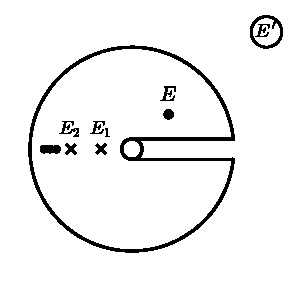
\includegraphics[width=4.2cm]{fig46.pdf}\\[0.3em]{\small 图 46}\end{minipage}\par\nopagebreak

另一方面，根据柯西定理，积分式(129.4)应等于 $f(0,E)-f_{\mathrm{B}}$ 再加上被积函数 $\dfrac{f(0,E')}{E'-E}$ 在各极点 $E'=E_n$ 处的留数 $R_n$，其中的 $E_n$ 就是各个离散能级的能量，这些留数可以用(128.17)式确定并等于
\begin{equation}
  R_n=\frac{d_n}{E_n-E},\qquad
  d_n=-(-1)^{l_n}(2l_n+1)\frac{\hbar^2A_{0n}^2}{2m},
\end{equation}
$l_n$ 是能量为 $E_n$ 的状态的角动量.因此得
\begin{equation}
  f(0,E)=f_{\mathrm{B}}
  +\frac{1}{\pi}\int_0^{\infty}
  \frac{\operatorname{Im}f(0,E')}{E'-E}\,\mathrm{d}E'
  +\sum_n\frac{d_n}{E-E_n}.
\end{equation}
此式称为色散关系，它用 $E>0$ 的 $f(0,E)$ 的虚部值确定物理叶上任一点的 $f(0,E)$ 值（D.~Y.~Wong, 1957; N.~Khuri, 1957）.

\par\nopagebreak\noindent\begin{minipage}{\linewidth}\centering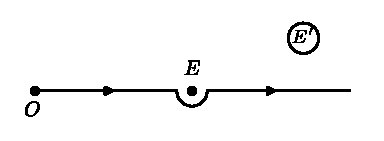
\includegraphics[width=5cm]{fig47.pdf}\\[0.3em]{\small 图 47}\end{minipage}\par\nopagebreak

当 $E$ 点趋于割线的上沿时，(129.6)式中沿实轴的积分应从下面绕过 $E=E'$ 极点，如果作一个无限小的半圆绕过这一点（图47），(129.6)式右边积分的相应部分给出 $\mathrm{i}\operatorname{Im}f(0,E)$，剩下从 0 到 $\infty$ 的积分必须取作主值.结果得
\begin{equation}
  \operatorname{Re}f(0,E)=f_{\mathrm{B}}
  +\frac{1}{\pi}\mathrm{P}\int_0^{\infty}
  \frac{\operatorname{Im}f(0,E')}{E'-E}\,\mathrm{d}E'
  +\sum_n\frac{d_n}{E-E_n},
\end{equation}
$E>0$ 的零角度散射振幅的实部就可以通过它的虚部来确定.可以提及的是，根据(125.9)式，后者直接和总散射截面相联系.

\section{动量表象中的散射振幅}

散射振幅的概念中只含有散射粒子的初末态动量的方向.因此自然地也能在动量表象中表述散射问题，在此表象中并不存在过程的空间分布问题.下面我们来看怎样做到这一点.

首先，我们取原来的薛定谔方程
\begin{equation}
  -\frac{\hbar^2}{2m}\nabla^2\psi(\boldsymbol{r})
  +\left[U(\boldsymbol{r})-E\right]\psi(\boldsymbol{r})=0,
\end{equation}
把坐标波函数变到动量表象，亦即变成它的傅里叶分量
\begin{equation}
  a(\boldsymbol{q})=\int\psi(\boldsymbol{r})
  \mathrm{e}^{-\mathrm{i}\boldsymbol{q}\cdot\boldsymbol{r}}\,\mathrm{d}V,
\end{equation}
反之有
\begin{equation}
  \psi(\boldsymbol{r})=\frac{1}{(2\pi)^3}\int a(\boldsymbol{q})
  \mathrm{e}^{\mathrm{i}\boldsymbol{q}\cdot\boldsymbol{r}}\,\mathrm{d}^3\boldsymbol{q}.
\end{equation}
(130.1)式乘以 $\mathrm{e}^{-\mathrm{i}\boldsymbol{q}\cdot\boldsymbol{r}}$ 并对 $\mathrm{d}V$ 积分.第一项作两次分部积分后给出
\begin{equation*}
  \int\mathrm{e}^{-\mathrm{i}\boldsymbol{q}\cdot\boldsymbol{r}}
  \nabla^2\psi(\boldsymbol{r})\,\mathrm{d}V
  =\int\psi(\boldsymbol{r})
  \nabla^2\mathrm{e}^{-\mathrm{i}\boldsymbol{q}\cdot\boldsymbol{r}}\,\mathrm{d}V
  =-q^2a(\boldsymbol{q}).
\end{equation*}
第二项中，$\psi(\boldsymbol{r})$ 用(130.3)代入，我们得
\begin{equation*}
\begin{aligned}
  \int U(\boldsymbol{r})\psi(\boldsymbol{r})
  \mathrm{e}^{-\mathrm{i}\boldsymbol{q}\cdot\boldsymbol{r}}\,\mathrm{d}V
  &=\iint U(\boldsymbol{r})\mathrm{e}^{-\mathrm{i}\boldsymbol{q}\cdot\boldsymbol{r}}
  a(\boldsymbol{q}')\mathrm{e}^{\mathrm{i}\boldsymbol{q}'\cdot\boldsymbol{r}}\,
  \mathrm{d}V\frac{\mathrm{d}^3q'}{(2\pi)^3}=\\
  &=\int U(\boldsymbol{q}-\boldsymbol{q}')a(\boldsymbol{q}')
  \frac{\mathrm{d}^3q'}{(2\pi)^3},
\end{aligned}
\end{equation*}
式中的 $U(\boldsymbol{q})$ 是场 $U(\boldsymbol{r})$ 的傅里叶分量\footnote{为方便计，我们把 $q$ 写成为傅里叶分量的宗量，不作下标处理.}
\begin{equation*}
  U(\boldsymbol{q})=\int U(\boldsymbol{r})
  \mathrm{e}^{-\mathrm{i}\boldsymbol{q}\cdot\boldsymbol{r}}\,\mathrm{d}V,
\end{equation*}
因此薛定谔方程在动量表象中变成
\begin{equation}
  \left(\frac{\hbar^2q^2}{2m}-E\right)a(\boldsymbol{q})
  +\int U(\boldsymbol{q}-\boldsymbol{q}')a(\boldsymbol{q}')
  \frac{\mathrm{d}^3q'}{(2\pi)^3}=0,
\end{equation}
注意这是一个积分方程，不是微分方程.

描述动量为 $\hbar\boldsymbol{k}$ 的粒子散射的波函数具有以下形式：
\begin{equation}
  \psi_{\boldsymbol{k}}(\boldsymbol{r})
  =\mathrm{e}^{\mathrm{i}\boldsymbol{k}\cdot\boldsymbol{r}}
  +\chi_{\boldsymbol{k}}(\boldsymbol{r}),
\end{equation}
式中的 $\chi_{\boldsymbol{k}}(\boldsymbol{r})$ 函数，它的渐近式（$r\to\infty$ 时）是一个射出球面波.上式的傅里叶分量为
\begin{equation}
  a_{\boldsymbol{k}}(\boldsymbol{q})=(2\pi)^3
  \delta(\boldsymbol{q}-\boldsymbol{k})+\chi_{\boldsymbol{k}}(\boldsymbol{q})
\end{equation}
此式代入(130.4)，得 $\chi_{\boldsymbol{k}}(\boldsymbol{q})$ 函数的以下方程\footnote{根据 $\delta$ 函数的性质，乘积 $(q^2-k^2)\delta(\boldsymbol{q}-\boldsymbol{k})$ 乘任一函数 $f(\boldsymbol{q})$（在 $\boldsymbol{q}=\boldsymbol{k}$ 处无奇点）后对 $\mathrm{d}^3q$ 积分等于零.在这个意义下，可令 $(q^2-k^2)\delta(\boldsymbol{q}-\boldsymbol{k})\equiv0$.}：
\begin{equation}
  \frac{\hbar^2}{2m}(k^2-q^2)\chi_{\boldsymbol{k}}(\boldsymbol{q})
  =U(\boldsymbol{q}-\boldsymbol{k})
  +\int U(\boldsymbol{q}-\boldsymbol{q}')\chi_{\boldsymbol{k}}(\boldsymbol{q}')
  \frac{\mathrm{d}^3q'}{(2\pi)^3}.
\end{equation}
用下式定义的未知函数代替 $\chi_{\boldsymbol{k}}(\boldsymbol{q})$，对上式进行变换：
\begin{equation}
  \chi_{\boldsymbol{k}}(\boldsymbol{q})=\frac{2m}{\hbar^2}
  \frac{F(\boldsymbol{k},\boldsymbol{q})}{q^2-k^2-\mathrm{i}0},
\end{equation}
这就消去了(130.7)式系数中 $q^2=k^2$ 处的奇点，该式变成
\begin{equation}
  F(\boldsymbol{k},\boldsymbol{q})=-U(\boldsymbol{q}-\boldsymbol{k})
  -\frac{2m}{\hbar^2}\int
  \frac{U(\boldsymbol{q}-\boldsymbol{q}')F(\boldsymbol{k},\boldsymbol{q}')}{q'^2-k^2-\mathrm{i}0}
  \frac{\mathrm{d}^3q'}{(2\pi)^3},
\end{equation}
其中的 $\mathrm{i}0$ 代表 $\delta\to+0$ 时 $\mathrm{i}\delta$ 的极值，它包括在定义(130.8)中，目的是使(130.9)式的积分具有给定的意义，因为它确立了绕过 $q^2=k^2$ 点的方式（参考§43）.我们来证明，这样的积分方式相当于使以下函数具有所需要的渐近形式：
\begin{equation}
  \chi_{\boldsymbol{k}}(\boldsymbol{r})=\frac{2m}{\hbar^2}\int
  \frac{F(\boldsymbol{k},\boldsymbol{q})
  \mathrm{e}^{\mathrm{i}\boldsymbol{q}\cdot\boldsymbol{r}}}{q^2-k^2-\mathrm{i}0}
  \frac{\mathrm{d}^3q}{(2\pi)^3}.
\end{equation}
为此，我们令 $\mathrm{d}^3q=q^2\mathrm{d}q\,\mathrm{d}o_q$ 并先对 $\mathrm{d}o_q$ 积分，即对矢量 $\boldsymbol{q}$ 相对于 $r$ 的各个方向积分.这类积分早已在(125.2)第一项的变换中做过；在 $r$ 大的区域内，结果是
\begin{equation*}
  \chi_{\boldsymbol{k}}(r)=-\frac{2m}{\hbar^2}\frac{2\pi\mathrm{i}}{r}
  \int_0^{\infty}
  \frac{F(\boldsymbol{k},q\boldsymbol{n}')\mathrm{e}^{\mathrm{i}qr}
  -F(\boldsymbol{k},-q\boldsymbol{n}')\mathrm{e}^{-\mathrm{i}qr}}
  {q^2-k^2-\mathrm{i}0}
  \frac{q\,\mathrm{d}q}{(2\pi)^3}
\end{equation*}
其中 $\boldsymbol{n}'=\boldsymbol{r}/r$，或者
\begin{equation*}
  \chi_{\boldsymbol{k}}(r)=-\frac{\mathrm{i}m}{2\pi^2\hbar^2r}
  \int_{-\infty}^{\infty}
  \frac{F(\boldsymbol{k},q\boldsymbol{n}')\mathrm{e}^{\mathrm{i}qr}\,q\,\mathrm{d}q}
  {q^2-k^2-\mathrm{i}0}.
\end{equation*}
被积函数在 $q=k+\mathrm{i}0$ 和 $q=-k-\mathrm{i}0$ 处具有极点；$q$ 复平面上的积分路线分别从下面和从上面绕过这两点（图48a）.这条积分路线可以稍为移动到上半平面内，用一条平行于实轴的直线和一个绕 $q=k$ 极点的封闭圈来代替（图48b）.

\par\nopagebreak\noindent\begin{minipage}{\linewidth}\centering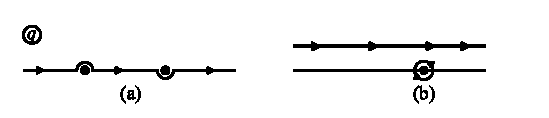
\includegraphics[width=9cm]{fig48.pdf}\\[0.3em]{\small 图 48}\end{minipage}\par\nopagebreak

沿直线的积分当 $r\to\infty$ 时趋于零（因为被积函数中含有
$\mathrm{e}^{-r\operatorname{Im}q}$ 因子），沿封闭圈的积分等于被积函数在极点 $q=k$ 处的留数乘以 $2\pi\mathrm{i}$.最后结果为
\begin{equation}
  \chi_{\boldsymbol{k}}(\boldsymbol{r})=\frac{m}{2\pi\hbar^2}
  \frac{\mathrm{e}^{\mathrm{i}kr}}{r}F(k\boldsymbol{n},k\boldsymbol{n}'),
\end{equation}
式中 $n$ 为 $\boldsymbol{k}$ 方向的单位矢量.我们已经导出了所需的波函数渐近式，而散射振幅为
\begin{equation}
  f(\boldsymbol{n},\boldsymbol{n}')
  =\frac{m}{2\pi\hbar^2}F(k\boldsymbol{n},k\boldsymbol{n}').
\end{equation}
可见散射振幅由满足积分方程(130.9)的 $F(\boldsymbol{k},\boldsymbol{q})$ 函数在 $q=k$ 点的值所决定.

当微扰论能用时，(130.9)式很易用叠代法求解.一级近似中略去积分项，我们有
$F(\boldsymbol{k},\boldsymbol{q})=-U(\boldsymbol{q}-\boldsymbol{k})$.
下一级近似中我们把它代入积分项内，(130.12)式的散射振幅就变成（稍改记号）
\begin{equation}
  f(\boldsymbol{n},\boldsymbol{n}')
  =-\frac{m}{2\pi\hbar^2}\left\{U(\boldsymbol{k}'-\boldsymbol{k})
  +\frac{2m}{\hbar^2}\int
  \frac{U(\boldsymbol{k}'-\boldsymbol{k}'')U(\boldsymbol{k}''-\boldsymbol{k})}
  {k^2-k''^2+\mathrm{i}0}
  \frac{\mathrm{d}^3k''}{(2\pi)^3}\right\},
\end{equation}
其中 $\boldsymbol{k}=k\boldsymbol{n}$，$\boldsymbol{k}'=k\boldsymbol{n}'$.第一项与一级近似(126.4)相同；第二项表明二级近似对散射振幅的贡献\footnote{这个结果不用动量表象当然也很易得到.二级近似与一级近似式的差别在于把(130.13)中大括号内的表式改成 $U(\boldsymbol{k}'-\boldsymbol{k})$，这可从(43.1)和(43.6)式的比较中明显看出.}.

从(130.13)可得§126中提到的一个结论：即使在二级近似中，散射振幅也已失去(126.8)式的对称性.初看起来，(130.13)的积分项对初末态的对调似乎也是对称的.实际不然，因为取复共轭表式后，积分路线及其绕过极点的方式已被改变.

\section{高能散射}

如果势能与 $\hbar^2/ma^2$（$a$ 和通常一样是势场的作用距离）相比并不小，就有可能发生一种情况，此时散射粒子的能量很大，使得
\begin{equation}
  |U|\ll E\sim\frac{\hbar^2}{ma^2}(ka)^2,
\end{equation}
但还满足条件
\begin{equation}
  |U|\gtrsim\frac{\hbar^2}{ma^2}ka=\frac{\hbar v}{a};
\end{equation}
当然，我们假定了
\begin{equation}
  ka\gg1.
\end{equation}
在这种情形下，虽是快粒子散射，但玻恩近似不适用：条件(126.1)和(126.2)都不满足.

考察这种情形，我们可用(45.9)的波函数表式：
\begin{equation}
  \psi=\mathrm{e}^{\mathrm{i}kz}F(r),\qquad
  F(r)=\exp\left(-\frac{\mathrm{i}}{\hbar v}\int_{-\infty}^{z}U\,\mathrm{d}z\right).
\end{equation}
应用此式时，能量只需满足条件 $|U|\ll E$.§45中曾经指出，上式只对 $z\ll ka^2$ 成立，所以它不能立即延伸到渐近式(123.3)得以成立的距离处.可是我们并不需要这样做；计算散射振幅时，知道 $a\ll z\ll ka^2$ 区间内的波函数已经足够，此时 $F(\boldsymbol{r})$ 指数中的积分可以延伸到无穷远：
\begin{equation}
  \psi=\mathrm{e}^{\mathrm{i}kz}S(\boldsymbol{\rho}),
\end{equation}
其中的记号
\begin{equation}
  S(\boldsymbol{\rho})=\mathrm{e}^{2\mathrm{i}\delta(\boldsymbol{\rho})},
  \qquad
  \delta(\boldsymbol{\rho})=-\frac{1}{2\hbar v}
  \int_{-\infty}^{\infty}U\,\mathrm{d}z,
\end{equation}
$\boldsymbol{\rho}$ 是 $xy$ 平面内的径矢.

快粒子散射主要发生在小角度，这是我们现在要考虑的.由于动量的改变 $\hbar\boldsymbol{q}$ 比较小（$q\ll k$），矢量 $\boldsymbol{q}$ 可以看成垂直于入射粒子的波矢 $\boldsymbol{k}$，也就是位于 $xy$ 平面内.散射波可从(131.5)减去入射波 $\mathrm{e}^{\mathrm{i}kz}$（$z=-\infty$ 的(131.4)式）后得到.波矢为 $\boldsymbol{k}'=\boldsymbol{k}+\boldsymbol{q}$ 的散射振幅和散射波的相应傅里叶分量成正比\footnote{求散射振幅的这种方法类似于讨论夫琅禾费衍射（《场论》，§61）时所用的方法.衍射效应使得(131.4)对 $z\geqslant ka^2$ 不适用.}：
\begin{equation*}
  f\sim\int\left[S(\boldsymbol{\rho})-1\right]
  \mathrm{e}^{-\mathrm{i}\boldsymbol{q}\cdot\boldsymbol{\rho}}\,
  \mathrm{d}^2\boldsymbol{\rho}
\end{equation*}
（$\mathrm{d}^2\boldsymbol{\rho}=\mathrm{d}x\,\mathrm{d}y$）.这个表式中的比例系数可通过与玻恩近似极限情形的比较而导出（见下面）.

这个计算也可用一个不同的方法来进行，它能直接导出一个完全确定的表式.为此我们采用(129.2)并把(131.4)的 $\psi$ 代入.由于按(45.8)有
\begin{equation*}
  \frac{2m}{\hbar^2}UF=2\mathrm{i}k\frac{\partial F}{\partial z},
\end{equation*}
得散射振幅（$\mathrm{e}^{\mathrm{i}kR_0}/R_0$ 的系数）
\begin{equation*}
\begin{aligned}
  f&=\frac{k}{2\pi\mathrm{i}}\int\frac{\partial F}{\partial z}
  \mathrm{e}^{-\mathrm{i}\boldsymbol{q}\cdot\boldsymbol{\rho}}\,
  \mathrm{d}x\,\mathrm{d}y\,\mathrm{d}z=\\
  &=\frac{k}{2\pi\mathrm{i}}\int
  \left[F(z=\infty)-F(z=-\infty)\right]
  \mathrm{e}^{-\mathrm{i}\boldsymbol{q}\cdot\boldsymbol{\rho}}\,
  \mathrm{d}x\,\mathrm{d}y,
\end{aligned}
\end{equation*}
把 $F$ 的表式代入，最后得\footnote{两维情形下，$U(x,z)$ 场中的散射振幅由以下类似的公式确定：
\begin{equation*}
  f=\frac{1}{\mathrm{i}}\sqrt{\frac{k}{2\pi}}\int\left[S(x)-1\right]\mathrm{e}^{-\mathrm{i}qx}\,\mathrm{d}x.
  \tag{131.7a}
\end{equation*}
$|f|^2\mathrm{d}\theta$ 是沿 $y$ 轴单位长度内的散射截面，$\theta$ 为 $xz$ 平面内的散射角；尚可参考§126题6.}
\begin{equation}
  f=\frac{k}{2\pi\mathrm{i}}\int\left[S(\boldsymbol{\rho})-1\right]
  \mathrm{e}^{-\mathrm{i}\boldsymbol{q}\cdot\boldsymbol{\rho}}\,
  \mathrm{d}^2\boldsymbol{\rho}.
\end{equation}
如果能量很高，以致 $\delta\sim|U|a/\hbar v\ll1$，玻恩近似成立：展开 $S-1\approx2\mathrm{i}\delta$，由(131.7)得
\begin{equation*}
  f=-\frac{m}{2\pi\hbar^2}\int U
  \mathrm{e}^{-\mathrm{i}\boldsymbol{q}\cdot\boldsymbol{\rho}}\,
  \mathrm{d}^2\boldsymbol{\rho}\,\mathrm{d}z,
\end{equation*}
与(126.4)式一致.

应用光学定理(125.9)，我们可以(131.7)导出散射总截面.零角度的散射振幅就是 $q=0$ 的 $f$ 值.因此得
\begin{equation}
  \sigma=\int2\operatorname{Re}(1-S)\,\mathrm{d}^2\boldsymbol{\rho}
  =\int4\sin^2\delta(\boldsymbol{\rho})\,\mathrm{d}^2\boldsymbol{\rho}.
\end{equation}
被积函数可看作碰撞参量在 $\mathrm{d}^2\boldsymbol{\rho}$ 范围内的粒子散射截面\footnote{§152中，将给出被多粒子系统所散射的情形下(131.7)和(131.8)式的推广.}.

(131.7)式并没有预先假定势场是有心力场.对有心力场讲来，值得看一下怎样从精确的一般公式(123.11)直接导出此式.

根据条件(131.1)—(131.3)，散射中起主要作用的是角动量 $l$ 大的分波振幅.因此波函数满足准经典条件，我们可用(124.1)式的 $\delta_l$.令该式中 $r_0\approx l/k$，$r^2=z^2+l^2/k^2$，我们得
\begin{equation*}
  \delta_l\approx-\frac{m}{\hbar^2}\int_{l/k}^{\infty}
  \frac{U(r)\,\mathrm{d}r}{\sqrt{k^2-l^2/r^2}}
  =-\frac{m}{\hbar^2k}\int_0^{\infty}
  U\left(\sqrt{z^2+l^2/k^2}\right)\mathrm{d}z,
\end{equation*}
这与(131.6)中 $\rho=l/k$ 时的 $\delta(\boldsymbol{\rho})$ 值一致\footnote{准经典函数 $2\hbar\delta(\boldsymbol{\rho})$ 是粒子作经典轨道运动时由场 $U$ 所引起的作用量的改变量.对快速粒子，轨道可取直线，从而 $2\delta(\boldsymbol{\rho})$ 等于下面两个经典作用量积分之差
\begin{equation*}
  \int_{-\infty}^{\infty}\sqrt{k^2-\frac{2mU}{\hbar^2}}\,\mathrm{d}z-\int_{-\infty}^{\infty}k\,\mathrm{d}z
  \approx-\frac{m}{\hbar^2 k}\int_{-\infty}^{\infty}U\,\mathrm{d}z.
\end{equation*}
在这种意义下，此处的 $2\delta(\boldsymbol{\rho})$ 所起的作用类似于几何光学中程函的作用.散射理论中的这种近似因而常称作\textbf{程函近似}.但应强调指出，散射振幅并不还原成为它的准经典值，因为一般讲来，条件 $\theta l\gg1$ 和 $\delta_l\gg1$ 并不满足.}.其次，小角度（$\theta\ll1$）时 $l$ 大的勒让德多项式可取(49.6)的形式：
\begin{equation*}
  \mathrm{P}_l(\cos\theta)\approx\mathrm{J}_0(\theta l)
  =\frac{1}{2\pi}\int_0^{2\pi}
  \mathrm{e}^{-\mathrm{i}\theta l\cos\varphi}\,\mathrm{d}\varphi.
\end{equation*}
上式代入(123.11)并把求和（对大的 $l$）改成积分，我们得
\begin{equation}
  f=\frac{1}{\pi}\int\!\!\int_0^{2\pi}
  f_l\,\mathrm{e}^{-\mathrm{i}\theta l\cos\varphi}\,
  \mathrm{d}\varphi\, l\,\mathrm{d}l
  =\frac{k^2}{\pi}\int f_l\,
  \mathrm{e}^{-\mathrm{i}\boldsymbol{q}\cdot\boldsymbol{\rho}}\,
  \mathrm{d}^2\boldsymbol{\rho},
\end{equation}
式中 $q$ 和 $\boldsymbol{\rho}$ 为两维矢量，其大小为 $q=k\theta$，$\rho=l/k$.最后，把(123.15)的 $f_l$［式中 $\delta_l=\delta(l/k)$］代入，就回到(131.7)式.

对于有心力场中的散射，(131.7)式对 $xy$ 面内的极角 $\varphi$（$\mathrm{d}^2\boldsymbol{\rho}=\rho\,\mathrm{d}\rho\,\mathrm{d}\varphi$）积分后，变成
\begin{equation}
  f=-\mathrm{i}k\int\left\{\exp[2\mathrm{i}\delta(\rho)]-1\right\}
  \mathrm{J}_0(q\rho)\,\rho\,\mathrm{d}\rho,
\end{equation}
§126中已指出，玻恩近似不能适用于大角度的快速粒子散射，如果截面是一个指数式小量的话.这里给出的方法在这种条件下也不能适用.这样的情形实际上是准经典的，微扰论不能应用.

根据准经典近似的一般规则（参考§52，§53），按指数规律衰减的散射截面中，它的指数可以通过经典禁区中“复轨道”的研究来确定.\footnote{关于指数因子前的系数的讨论，见 А.~З.~Паташинский，В.~Л.~Покровский，И.~М.~Халатников，ЖЭТФ 45, 989, 1963（Soviet Physics JETP 18, 683, 1964）.}

经典散射问题中，粒子在场 $U(r)$ 中的散射角 $\theta$ 与碰撞参量 $\rho$ 之间的关系为
\begin{equation}
  \frac{\pi\pm\theta}{2}=\int_{r_0}^{\infty}
  \frac{\rho\,\mathrm{d}r}
  {r^2\sqrt{1-\dfrac{\rho^2}{r^2}-\dfrac{U}{E}}},
\end{equation}
$r_0$ 是最接近于力心的距离，为下式的一个根.
\begin{equation}
  1-\frac{\rho^2}{r^2}-\frac{U}{E}=0
\end{equation}
（见(127.5)）.我们感兴趣的情形相当于经典粒子散射中不能偏转的角度区\footnote{这里所讲的方法不但对大的 $E$ 成立，而且对散射为指数式小的所有情形都成立.}.这些角度相当于(131.11)式的复数解 $\rho(\theta)$（具有相应的 $r_0$ 复值）.根据这样求出的函数 $\rho(\theta)$ 以及粒子的经典轨道角动量 $mv\rho$，可以算出作用量
\begin{equation}
  S(\theta)=mv\int\rho(\theta)\,\mathrm{d}\theta,
\end{equation}
式中 $v$ 是粒子在无穷远处的速度.散射振幅为
\begin{equation}
  f\sim\exp\left(-\frac{1}{\hbar}\operatorname{Im}S(\theta)\right).
\end{equation}
一般讲来，(131.12)式的复根不止一个.(131.11)式中的 $r_0$ 应该选取这样的一个复根，它具有最小的正虚部 $\operatorname{Im}S$.此外，如果 $U(r)$ 具有复奇点，也应看作 $r_0$ 的一个可能值\footnote{我们记得（见§126），如果 $U(r)$ 当 $r$ 为实量时具有奇点.则截面不按指数规律衰减.}.

$r\sim r_0$ 区域在(131.11)的积分中最为重要.当 $E$ 很大时，根号内的 $U/E$ 项可以略去.积分后得
\begin{equation}
  \rho=r_0\cos\frac{1}{2}\theta.
\end{equation}
如果 $r_0$ 是函数 $U(r)$ 的一个奇点，它只和场的性质有关而和 $\rho$ 或 $E$ 无关.用(131.13)式算出 $S$ 后，即得这种情形下的散射振幅为
\begin{equation}
  f\sim\exp\left(-\frac{2mv}{\hbar}
  \sin\frac{\theta}{2}\operatorname{Im}r_0\right).
\end{equation}
但如 $r_0$ 取自(131.12)式的一个根，指数的形状就和场的特点有关.例如以下函数
\begin{equation*}
  U=U_0\mathrm{e}^{-(r/a)^2}
\end{equation*}
（它在有限距离内无奇点）根据方程式
\begin{equation*}
  \frac{U}{E}=1-\frac{\rho^2}{r^2}\approx\sin^2\frac{\theta}{2}
\end{equation*}
得
\begin{equation}
  r_0\approx\mathrm{i}a\sqrt{\ln\left(\frac{E}{U_0}\sin^2\frac{1}{2}\theta\right)}.
\end{equation}
由于它对 $\theta$ 的依赖性极小，$r_0$ 在(131.13)的积分中可以看作常数，结果得(131.16)式的散射振幅，其中的 $r_0$ 由(131.17)式给出.

\begin{xiti}

\noindent{\heiti 习题1}\quad 对半径为 $a$ 深度为 $U_0$ 并满足条件(131.1) $U_0\ll\hbar^2k^2/m$ 的球形方势阱，求总散射截面.

解：我们有
\begin{equation*}
  \int_{-\infty}^{\infty}U\,\mathrm{d}z=-2U_0\sqrt{a^2-\rho^2}.
\end{equation*}
根据(131.7)，向前散射振幅（$q=0$）为
\begin{equation*}
\begin{aligned}
  f(0)&=-\frac{\mathrm{i}k}{2\pi}\int_0^{a}
  \left[\exp\left(\frac{2\mathrm{i}U_0}{\hbar v}\sqrt{a^2-\rho^2}\right)-1\right]
  2\pi\rho\,\mathrm{d}\rho=\\
  &=-\mathrm{i}ka^2\int_0^{1}\left(\mathrm{e}^{2\mathrm{i}\nu x}-1\right)
  x\,\mathrm{d}x
  =\frac{ka^2}{2}\left[\mathrm{i}-\frac{\mathrm{e}^{2\mathrm{i}\nu}}{\nu}
  -\frac{\mathrm{i}}{2\nu^2}\left(\mathrm{e}^{2\mathrm{i}\nu}-1\right)\right],
\end{aligned}
\end{equation*}
其中 $\nu=U_0a/\hbar v$ 为“玻恩参量”.根据光学定理(125.9)，求得总截面：
\begin{equation*}
  \sigma=2\pi a^2\left[1+\frac{1}{2\nu^2}
  -\frac{\sin 2\nu}{\nu}-\frac{\cos 2\nu}{2\nu^2}\right]
\end{equation*}
在 $\nu\ll1$ 的（玻恩）极限情形下，上式给出 $\sigma=2\pi a^2\nu^2$，与§126题1一致.在 $\nu\gg1$ 的相反极限情形下，我们有 $\sigma=2\pi a^2$，即几何截面的两倍.后一结果具有简单的含义.当 $\nu\gg1$ 时，碰撞参量 $\rho<a$ 的所有粒子均被散射，亦即离开入射束.在这个意义下，势阱具有“吸收”球的行为；根据巴比涅（Babinet）原理（见《场论》§61末），总截面为“吸收”截面的两倍.

\noindent{\heiti 习题2}\quad 同题1，但场 $U=U_0\exp(-r^2/a^2)$.

解：这种情形下
\begin{equation*}
  \int_{-\infty}^{\infty}U\,\mathrm{d}z
  =a\sqrt{\pi}\,U_0\exp(-\rho^2/a^2),
\end{equation*}
代入(131.7)，改变积分变量，得零角度散射振幅
\begin{equation*}
  f(0)=-\frac{\mathrm{i}ka^2}{2}\int_0^{\nu\sqrt{\pi}}
  \left(\mathrm{e}^{-\mathrm{i}u}-1\right)\frac{\mathrm{d}u}{u},
\end{equation*}
式中 $\nu=U_0a/\hbar v$.故总截面为
\begin{equation*}
  \sigma=2\pi a^2\int_0^{\nu\sqrt{\pi}}
  (1-\cos u)\frac{\mathrm{d}u}{u}.
\end{equation*}
对于 $\nu\ll1$，被积函数为 $1/2u$，截面
$\sigma=\frac{1}{2}\pi^2a^2\nu^2$，
这与§126题2（$ka\gg1$ 时）一致.对于 $\nu\gg1$，我们把被积函数写成
$(1-\mathrm{e}^{-\lambda u}\cos u)/u$，含有一个小参量 $\lambda$，积分后再令它趋于零，分部积分后给出
\begin{equation*}
  \int_0^{\nu\sqrt{\pi}}(1-\cos u)\frac{\mathrm{d}u}{u}
  \approx\ln(\nu\sqrt{\pi})
  -\int_0^{\infty}\ln u\sin u\,\mathrm{d}u
  =\ln(\nu\sqrt{\pi})+C,
\end{equation*}
式中 $C$ 是欧拉常数.故
\begin{equation*}
  \sigma=2\pi a^2\ln\left|\nu\sqrt{\pi}\,\mathrm{e}^{C}\right|,
  \qquad\nu\gg1.
\end{equation*}

\noindent{\heiti 习题3}\quad 求磁场中电子小角度散射的截面，该场集中在半径为 $a$ 的柱形区内（Y.~Aharonov, D.~Bohm, 1959）.

解：令磁场沿 $y$ 轴，它也就是柱形区的轴，并取入射电子束的方向为 $z$ 轴.那么散射与坐标 $y$ 无关，我们可以考虑 $xz$ 平面内的两维问题.

柱形区外，磁场 $\boldsymbol{H}=0$，但其矢势不等于零：
\setcounter{equation}{0}\renewcommand{\theequation}{\arabic{equation}}%
\begin{equation}
  \boldsymbol{A}=\frac{\Phi}{2\pi}\nabla\varphi,
\end{equation}
式中 $\varphi$ 是 $xz$ 平面内的极角，$\Phi$ 是磁通量；实际上对 $xz$ 平面内的圆（半径 $r>a$）面积进行积分，即有
\begin{equation*}
  \int H\,\mathrm{d}x\,\mathrm{d}z
  =\oint\boldsymbol{A}\cdot\mathrm{d}\boldsymbol{l}
  =\frac{\Phi}{2\pi}\varphi\bigg|_0^{2\pi}=\Phi.
\end{equation*}
势(1)改变了电子波函数（平面波）的相位；按(111.9)，我们有
\begin{equation}
  \psi=\mathrm{e}^{\mathrm{i}kz}
  \exp\left(\frac{\mathrm{i}e}{\hbar c}\frac{\Phi}{2\pi}\varphi\right).
\end{equation}
但是此式在沿 $z>0$ 半轴的一个窄区（宽度 $\sim a$）内不适用，因为通过磁场区域的粒子运动受到了该场的干扰.这就解释了绕原点使 $\varphi$ 角增加 $2\pi$ 时函数(2)出现的非唯一性.实际上从(2)式的不适用性得到，在 $z>0$ 的半轴附近有一条割线（宽度为有限）：在割线的两侧，$\varphi$ 值相差 $2\pi$，例如 $\pm\pi$.

对于具有小动量转移 $q\approx k\theta$（$qa\ll1$，$\theta\ll1$）的小角度散射，横距 $x\sim1/q\gg a$ 是重要的，割线的宽度可以略去.考虑 $z\gg|x|$ 的区域，我们还能略去 $z$ 轴两侧 $\psi$ 对 $x$ 的依赖关系，得到\footnote{(3)和(131.4)式一样，对很大的 $z$ 值不适用，那时衍射效应变得很重要.}
\begin{equation}
  \psi=\mathrm{e}^{\mathrm{i}kz}F(x),\qquad
  F(x)=\left\{
  \begin{array}{ll}
    \exp\left(-\dfrac{\mathrm{i}e}{2\hbar c}\Phi\right), & x>0,\\[1em]
    \exp\left(\dfrac{\mathrm{i}e}{2\hbar c}\Phi\right), & x<0.
  \end{array}\right.
\end{equation}
“两维”散射振幅由(131.7a)式算出\footnote{早已提及，这个公式（$q=0$）不用势场中的薛定谔方程也能导出.}. $q\neq0$ 时我们有
\begin{equation*}
  f=\frac{1}{\mathrm{i}}\sqrt{\frac{k}{2\pi}}
  \left\{\exp\left(-\frac{\mathrm{i}e\Phi}{2\hbar c}\right)
  \int_0^{\infty}\mathrm{e}^{-\mathrm{i}qx}\,\mathrm{d}x
  +\text{复共轭式}\right\}
\end{equation*}
计算此积分时引入 $\mathrm{e}^{-\lambda x}$ 因子，积分后再令 $\lambda\to0$，结果为
\begin{equation*}
  f=\frac{\mathrm{i}}{q}\sqrt{\frac{2k}{\pi}}
  \sin\frac{e\Phi}{2\hbar c}
\end{equation*}
从而散射截面为
\begin{equation}
  \mathrm{d}\sigma=|f|^2\,\mathrm{d}\theta
  =\frac{2}{\pi k}\sin^2\frac{e\Phi}{2\hbar c}\,
  \frac{\mathrm{d}\theta}{\theta^2}
\end{equation}
$\dfrac{e\Phi}{\hbar c}\ll1$ 时，我们得
\begin{equation*}
  \mathrm{d}\sigma=\frac{e^2\Phi^2}{2\pi k\hbar^2c^2}
  \frac{\mathrm{d}\theta}{\theta^2}
\end{equation*}
相当于微扰论适用时的情形.

注意截面(4)和磁场强度具有周期性的依赖关系，并当 $\theta\to0$ 时总截面是发散的，尽管磁场是集中在一个有限的空间区域内.这些都是特有的量子效应.

\end{xiti}
\setcounter{equation}{0}\renewcommand{\theequation}{\arabic{section}.\arabic{equation}}%
